\begin{frame}[noframenumbering]
  \frametitle{V\&V Study 1: Verification of Moltres with the CNRS Benchmark}

  Published in \textit{S.M. Park, M. Munk, "Verification of Moltres for Multiphysics Simulations of
    Fast-Spectrum Molten Salt Reactors," Annals of Nuclear Energy, vol. 173, Aug 2022.}
  \vspace{.2cm}

  \begin{columns}
    \column[t]{6.5cm}
    \textbf{Description of the CNRS Benchmark \cite{tiberga_results_2020}}
    \vspace{.2cm}

      \begin{itemize}
        \item A numerical benchmark for multiphysics software dedicated to modeling ``pool-type''
          fast-spectrum MSRs
        \item Problem Setup
          \begin{itemize}
            \item LiF-BeF$_2$-UF$_4$ molten salt
            \item Six neutron energy groups
            \item Eight precursor groups
            \item Volumetric conjugate heat sink term
            \item Incompressible flow
          \end{itemize}
        \item Consists of three phases
          \begin{itemize}
            \item Phase 0: Single-physics verification
            \item Phase 1: Steady-state coupling
            \item Phase 2: Time-dependent coupling
          \end{itemize}
      \end{itemize}
    \column[t]{3.5cm}
    \begin{figure}
      \centering
      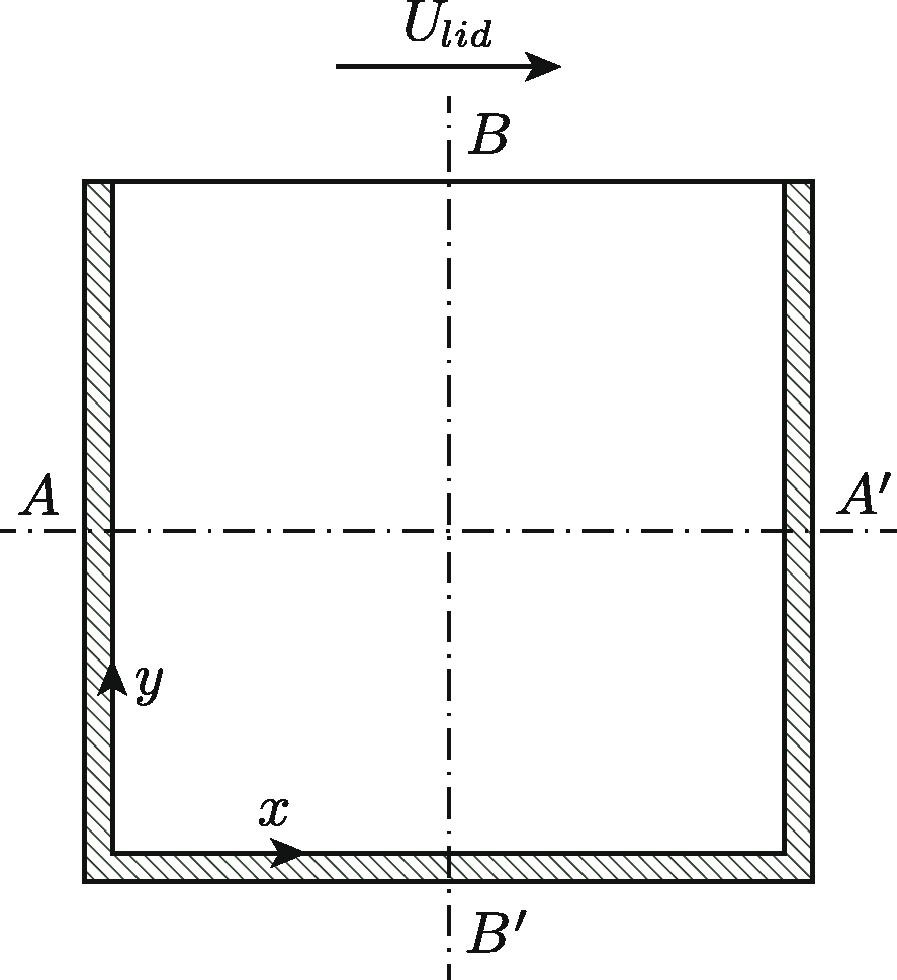
\includegraphics[width=\columnwidth]{../images/cnrs-geometry}
      \caption{CNRS benchmark problem domain \cite{tiberga_results_2020}}
    \end{figure}
  \end{columns}
\end{frame}

\begin{frame}[noframenumbering]
  \frametitle{V\&V Study 1: Verification of Moltres with the CNRS Benchmark}
  \begin{block}{\textbf{Study Outcome}}
    Moltres is consistent with the other multiphysics software in the benchmark problems.
  \end{block}
  \begin{columns}
    \hfill
    \column[t]{4cm}
    \vspace{.3cm}
    \begin{figure}
      \centering
      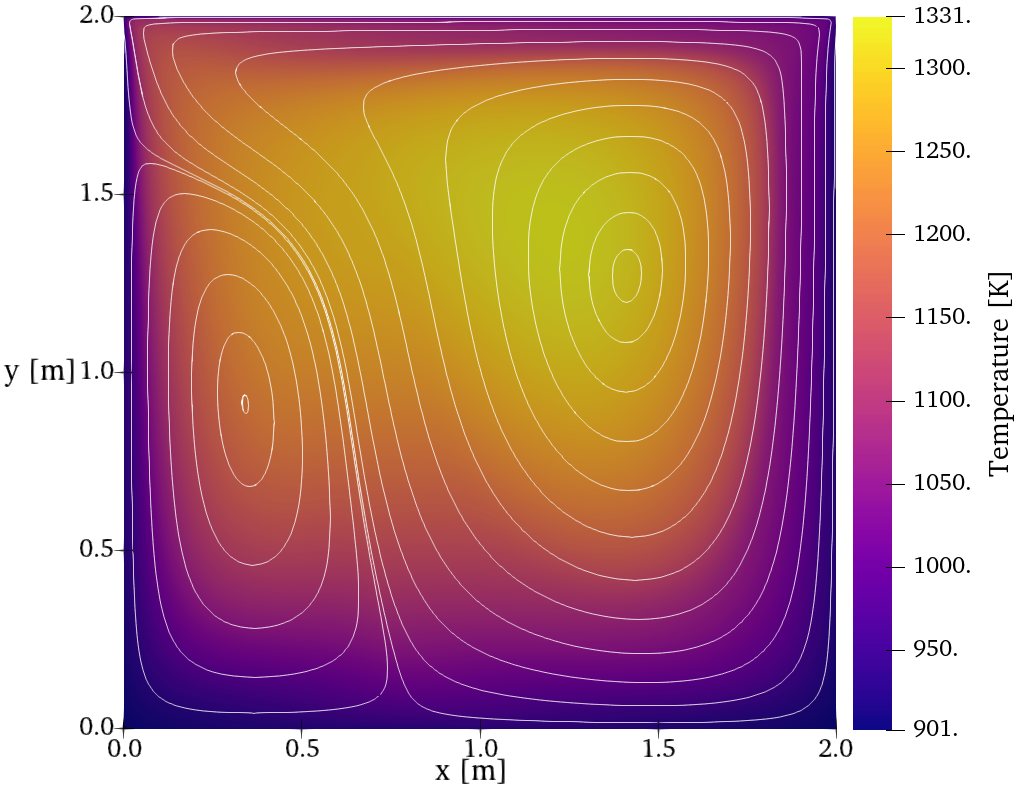
\includegraphics[width=\columnwidth]{../images/full-coupled}
      \caption{Step 1.4 - Temperature distribution and flow streamlines for the fully
      coupled system \cite{park_verification_2022}.}
    \end{figure}
    \column[t]{4cm}
    \begin{figure}
      \centering
      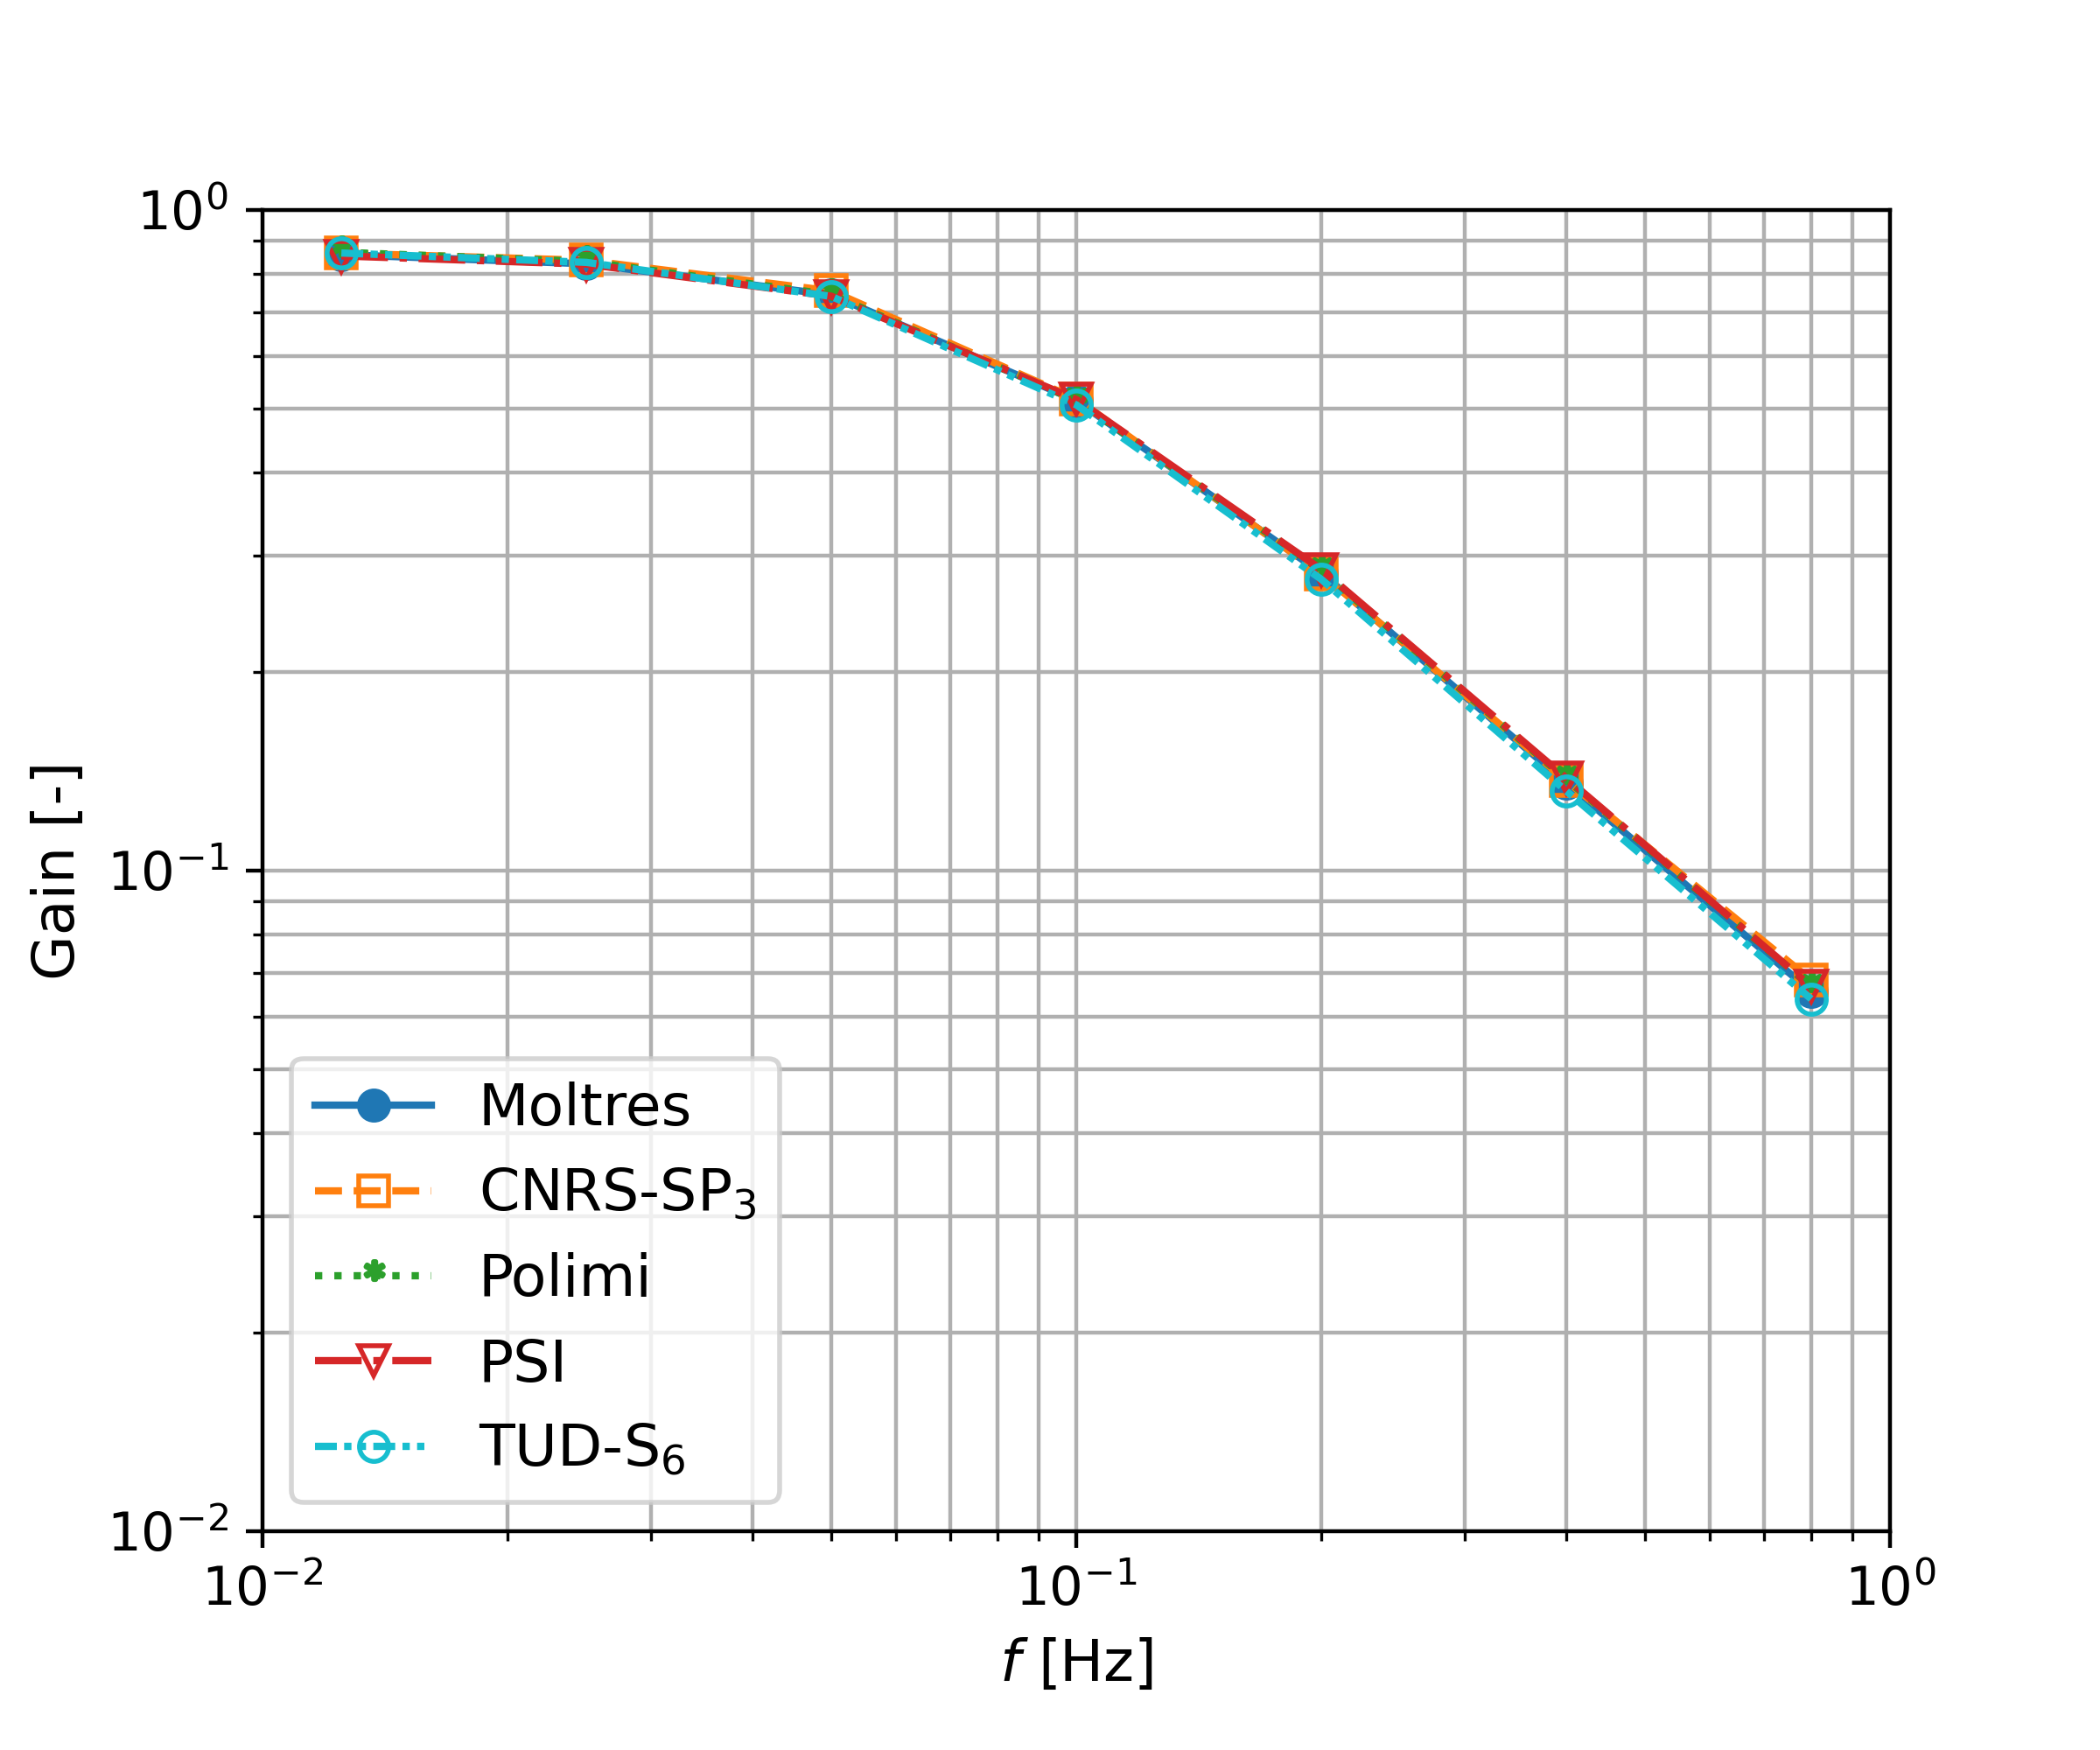
\includegraphics[width=\columnwidth]{../images/2-1-gain-plot}
      \caption{Step 2.1 - Bode gain plot of the frequency response of the fully
      coupled system \cite{park_verification_2022}.}
    \end{figure}
    \column[t]{4cm}
    \begin{figure}
      \centering
      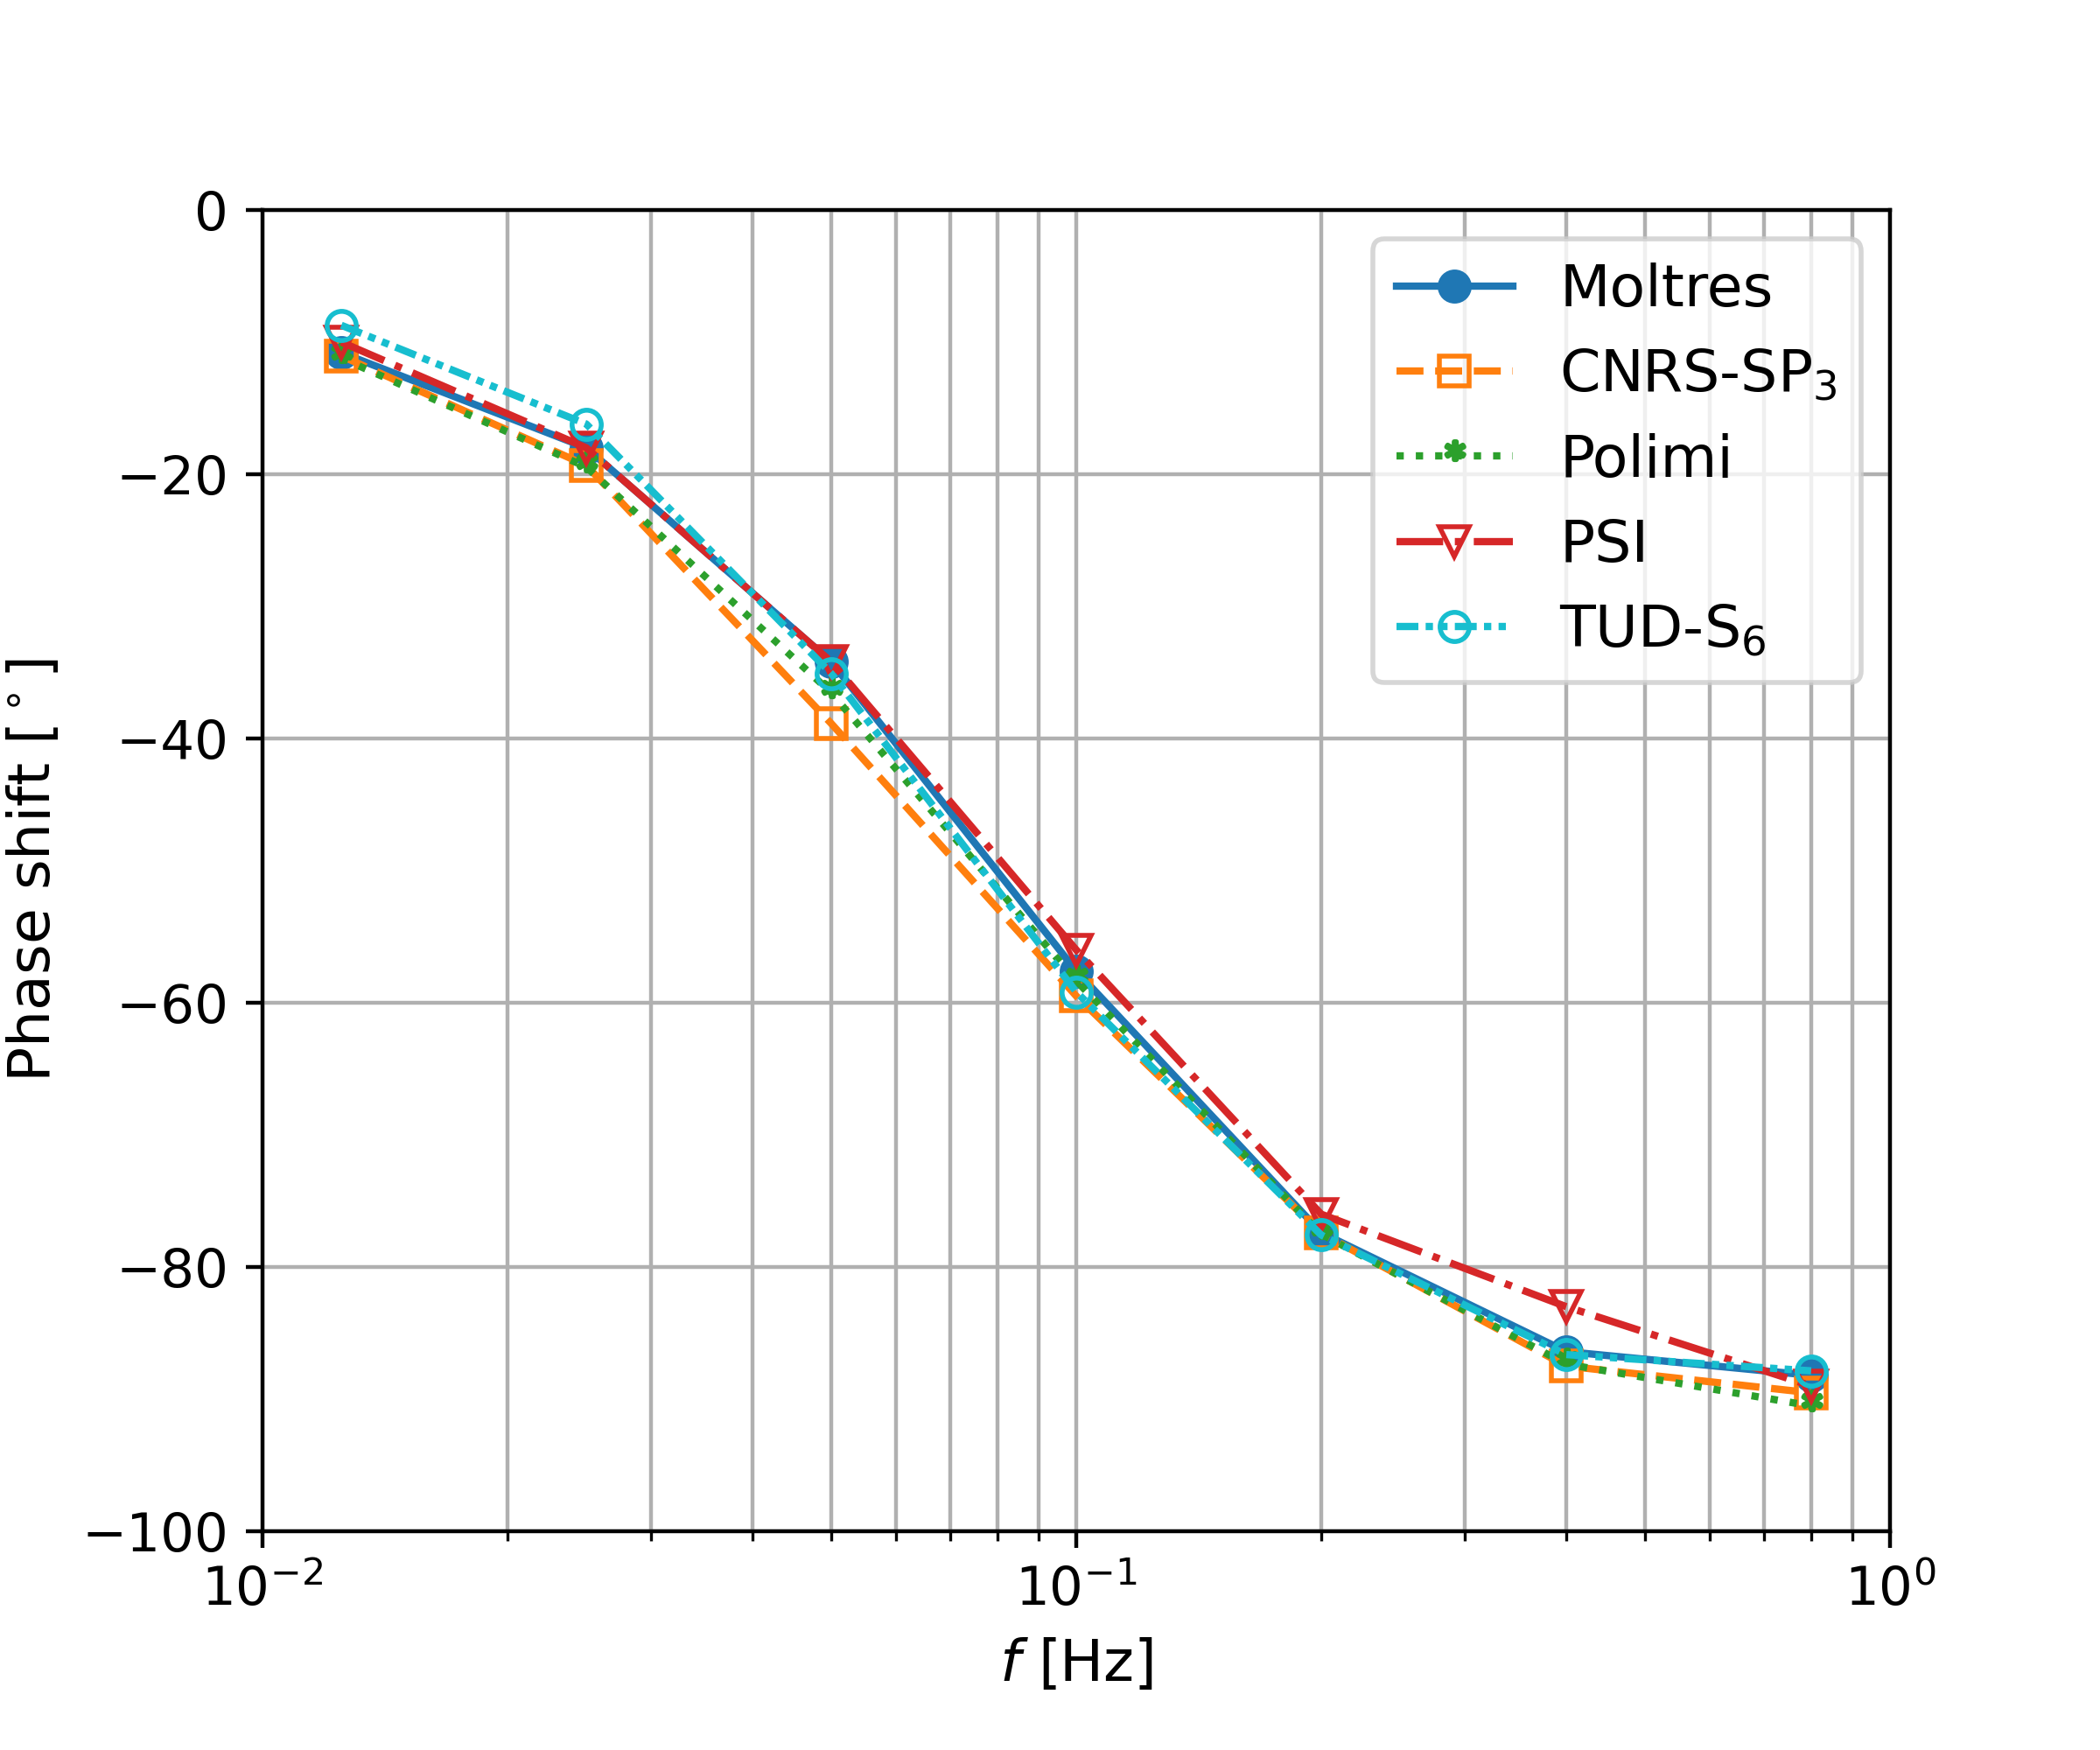
\includegraphics[width=\columnwidth]{../images/2-1-phase-plot}
      \caption{Step 2.1 - Bode phase plot of the frequency response of the fully
      coupled system \cite{park_verification_2022}.}
    \end{figure}
    \hfill
  \end{columns}
\end{frame}

\begin{frame}[noframenumbering]
  \frametitle{V\&V Study 2: MSRE Pump Start-up \& Coast-Down Transients}
  \textbf{DNP Distributions Under Static Conditions}
  \begin{figure}[t]
    \centering
    \begin{subfigure}[b]{0.48\columnwidth}
      \centering
      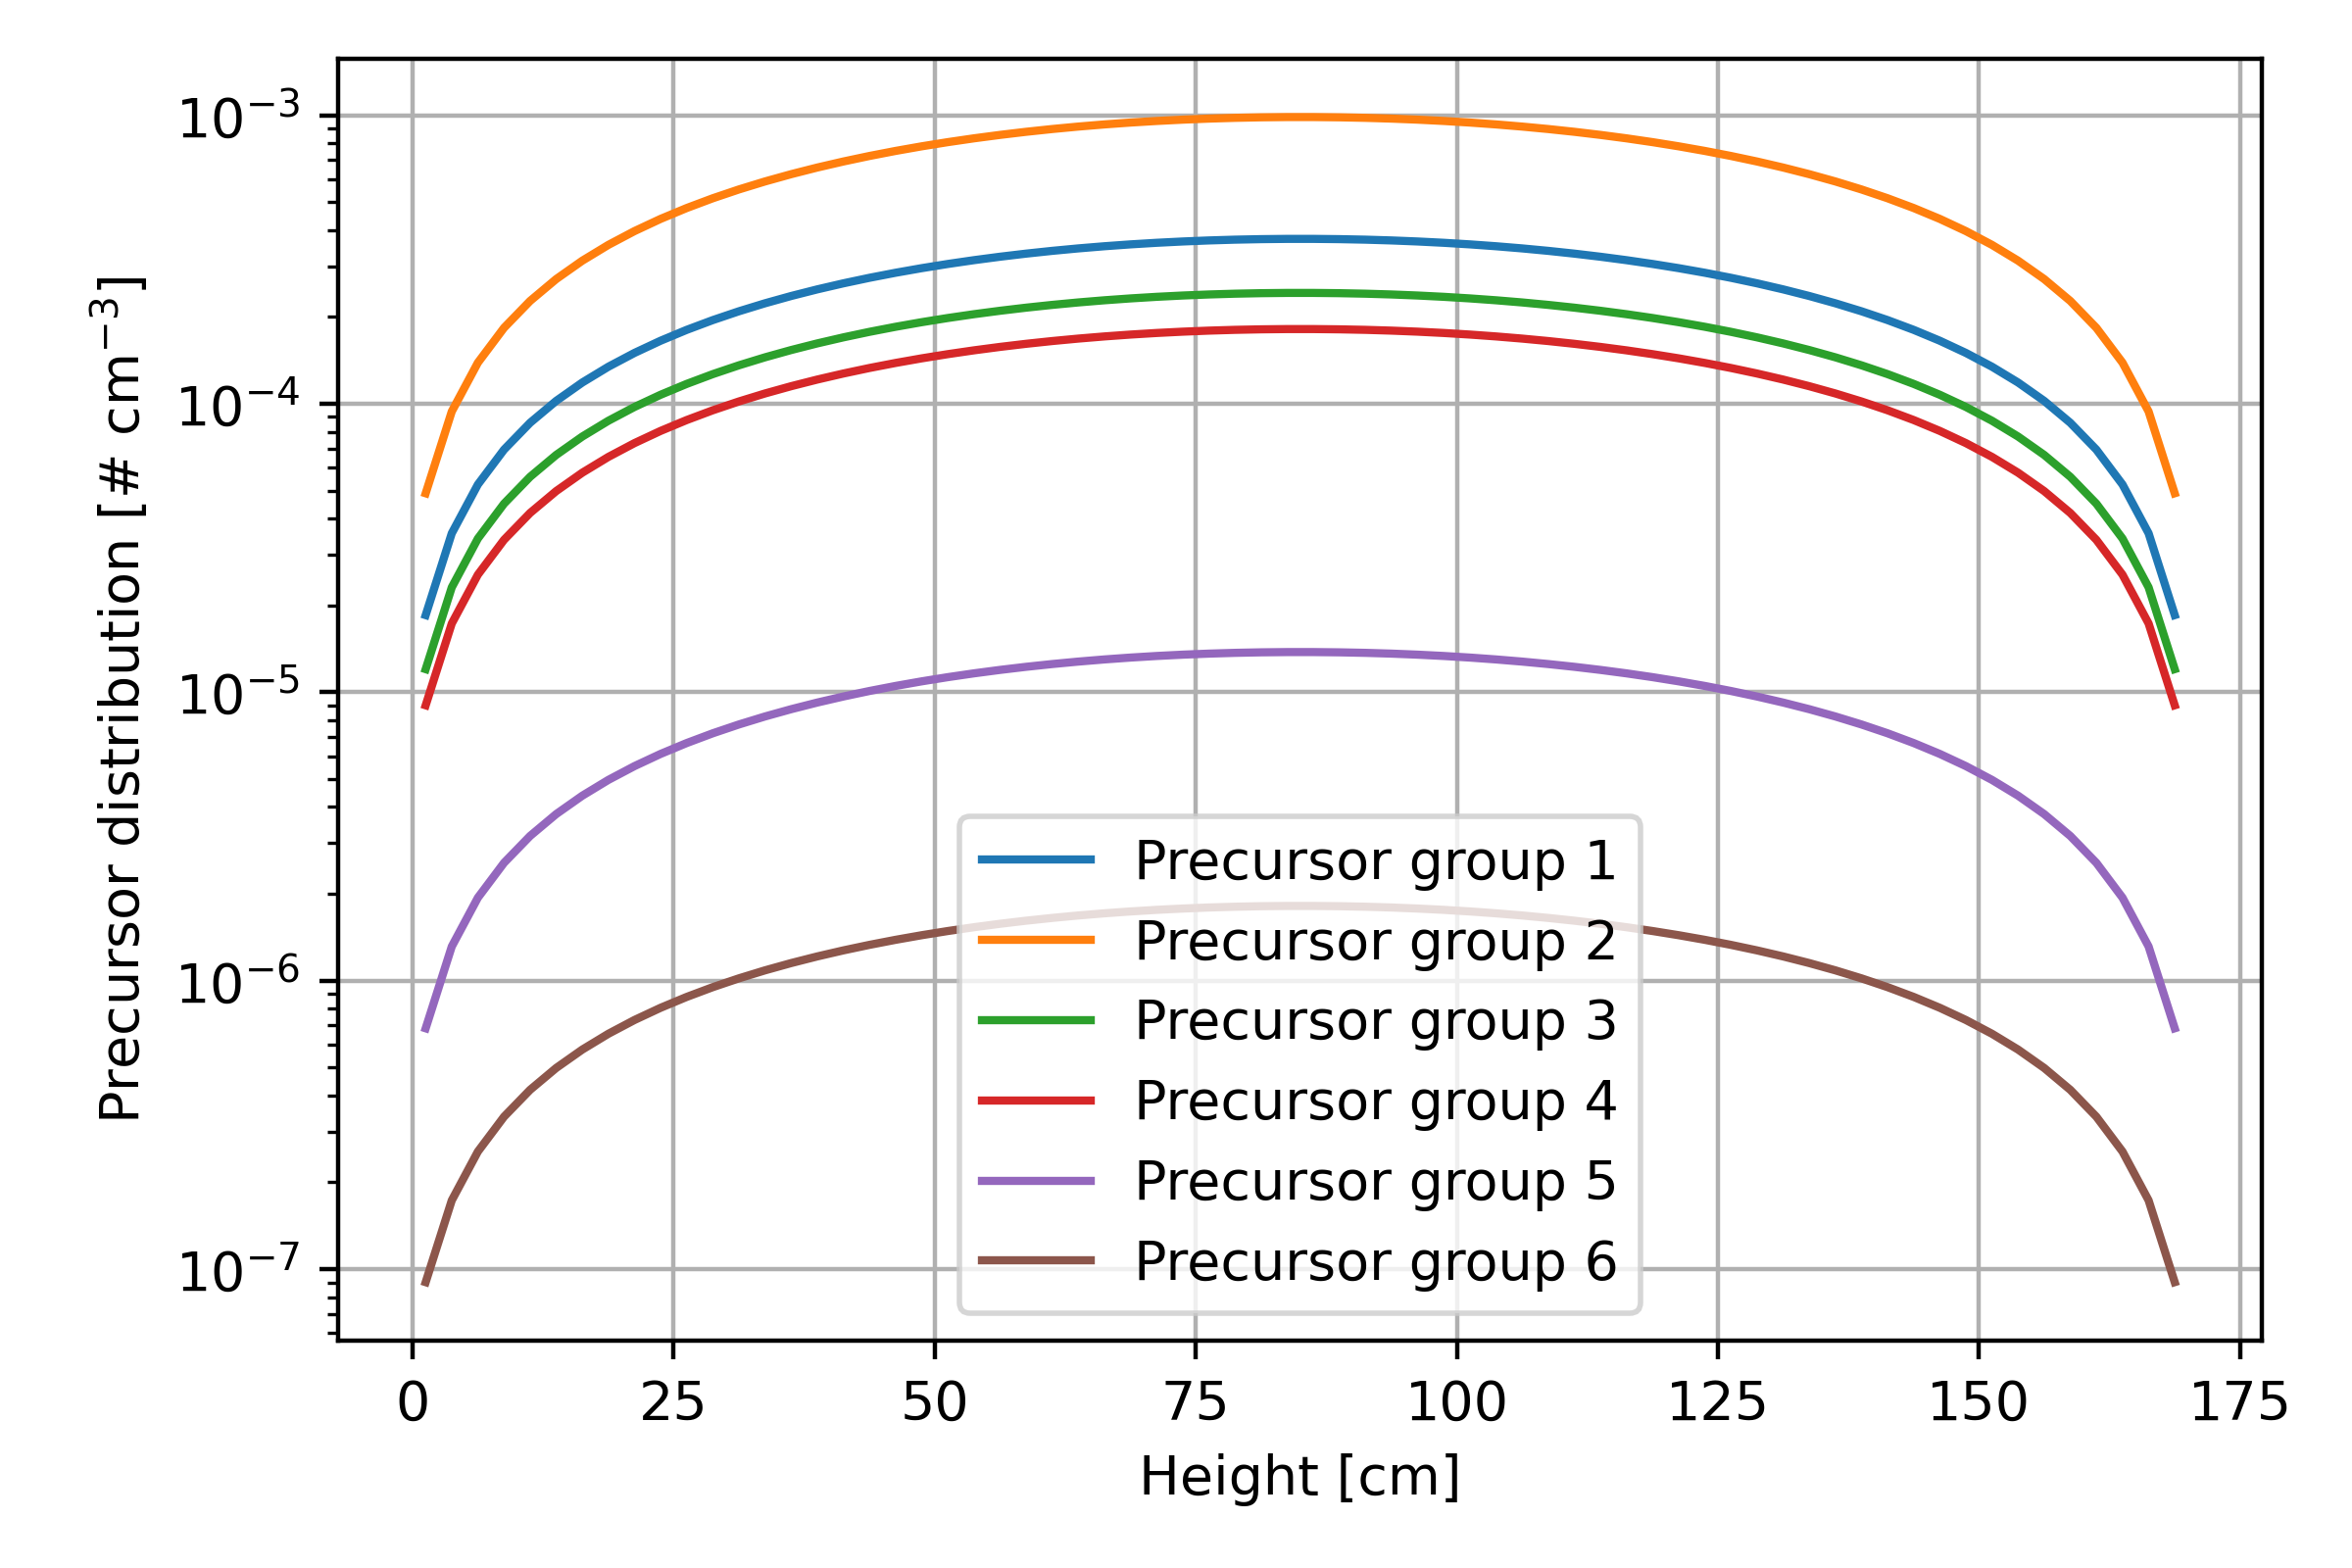
\includegraphics[width=\columnwidth]{centerline_pre}
      \caption{Normalized centerline \gls{DNP} distributions.}
      \label{fig:centerline-pre-dist}
    \end{subfigure}
    \hfill
    \begin{subfigure}[b]{0.48\columnwidth}
      \centering
      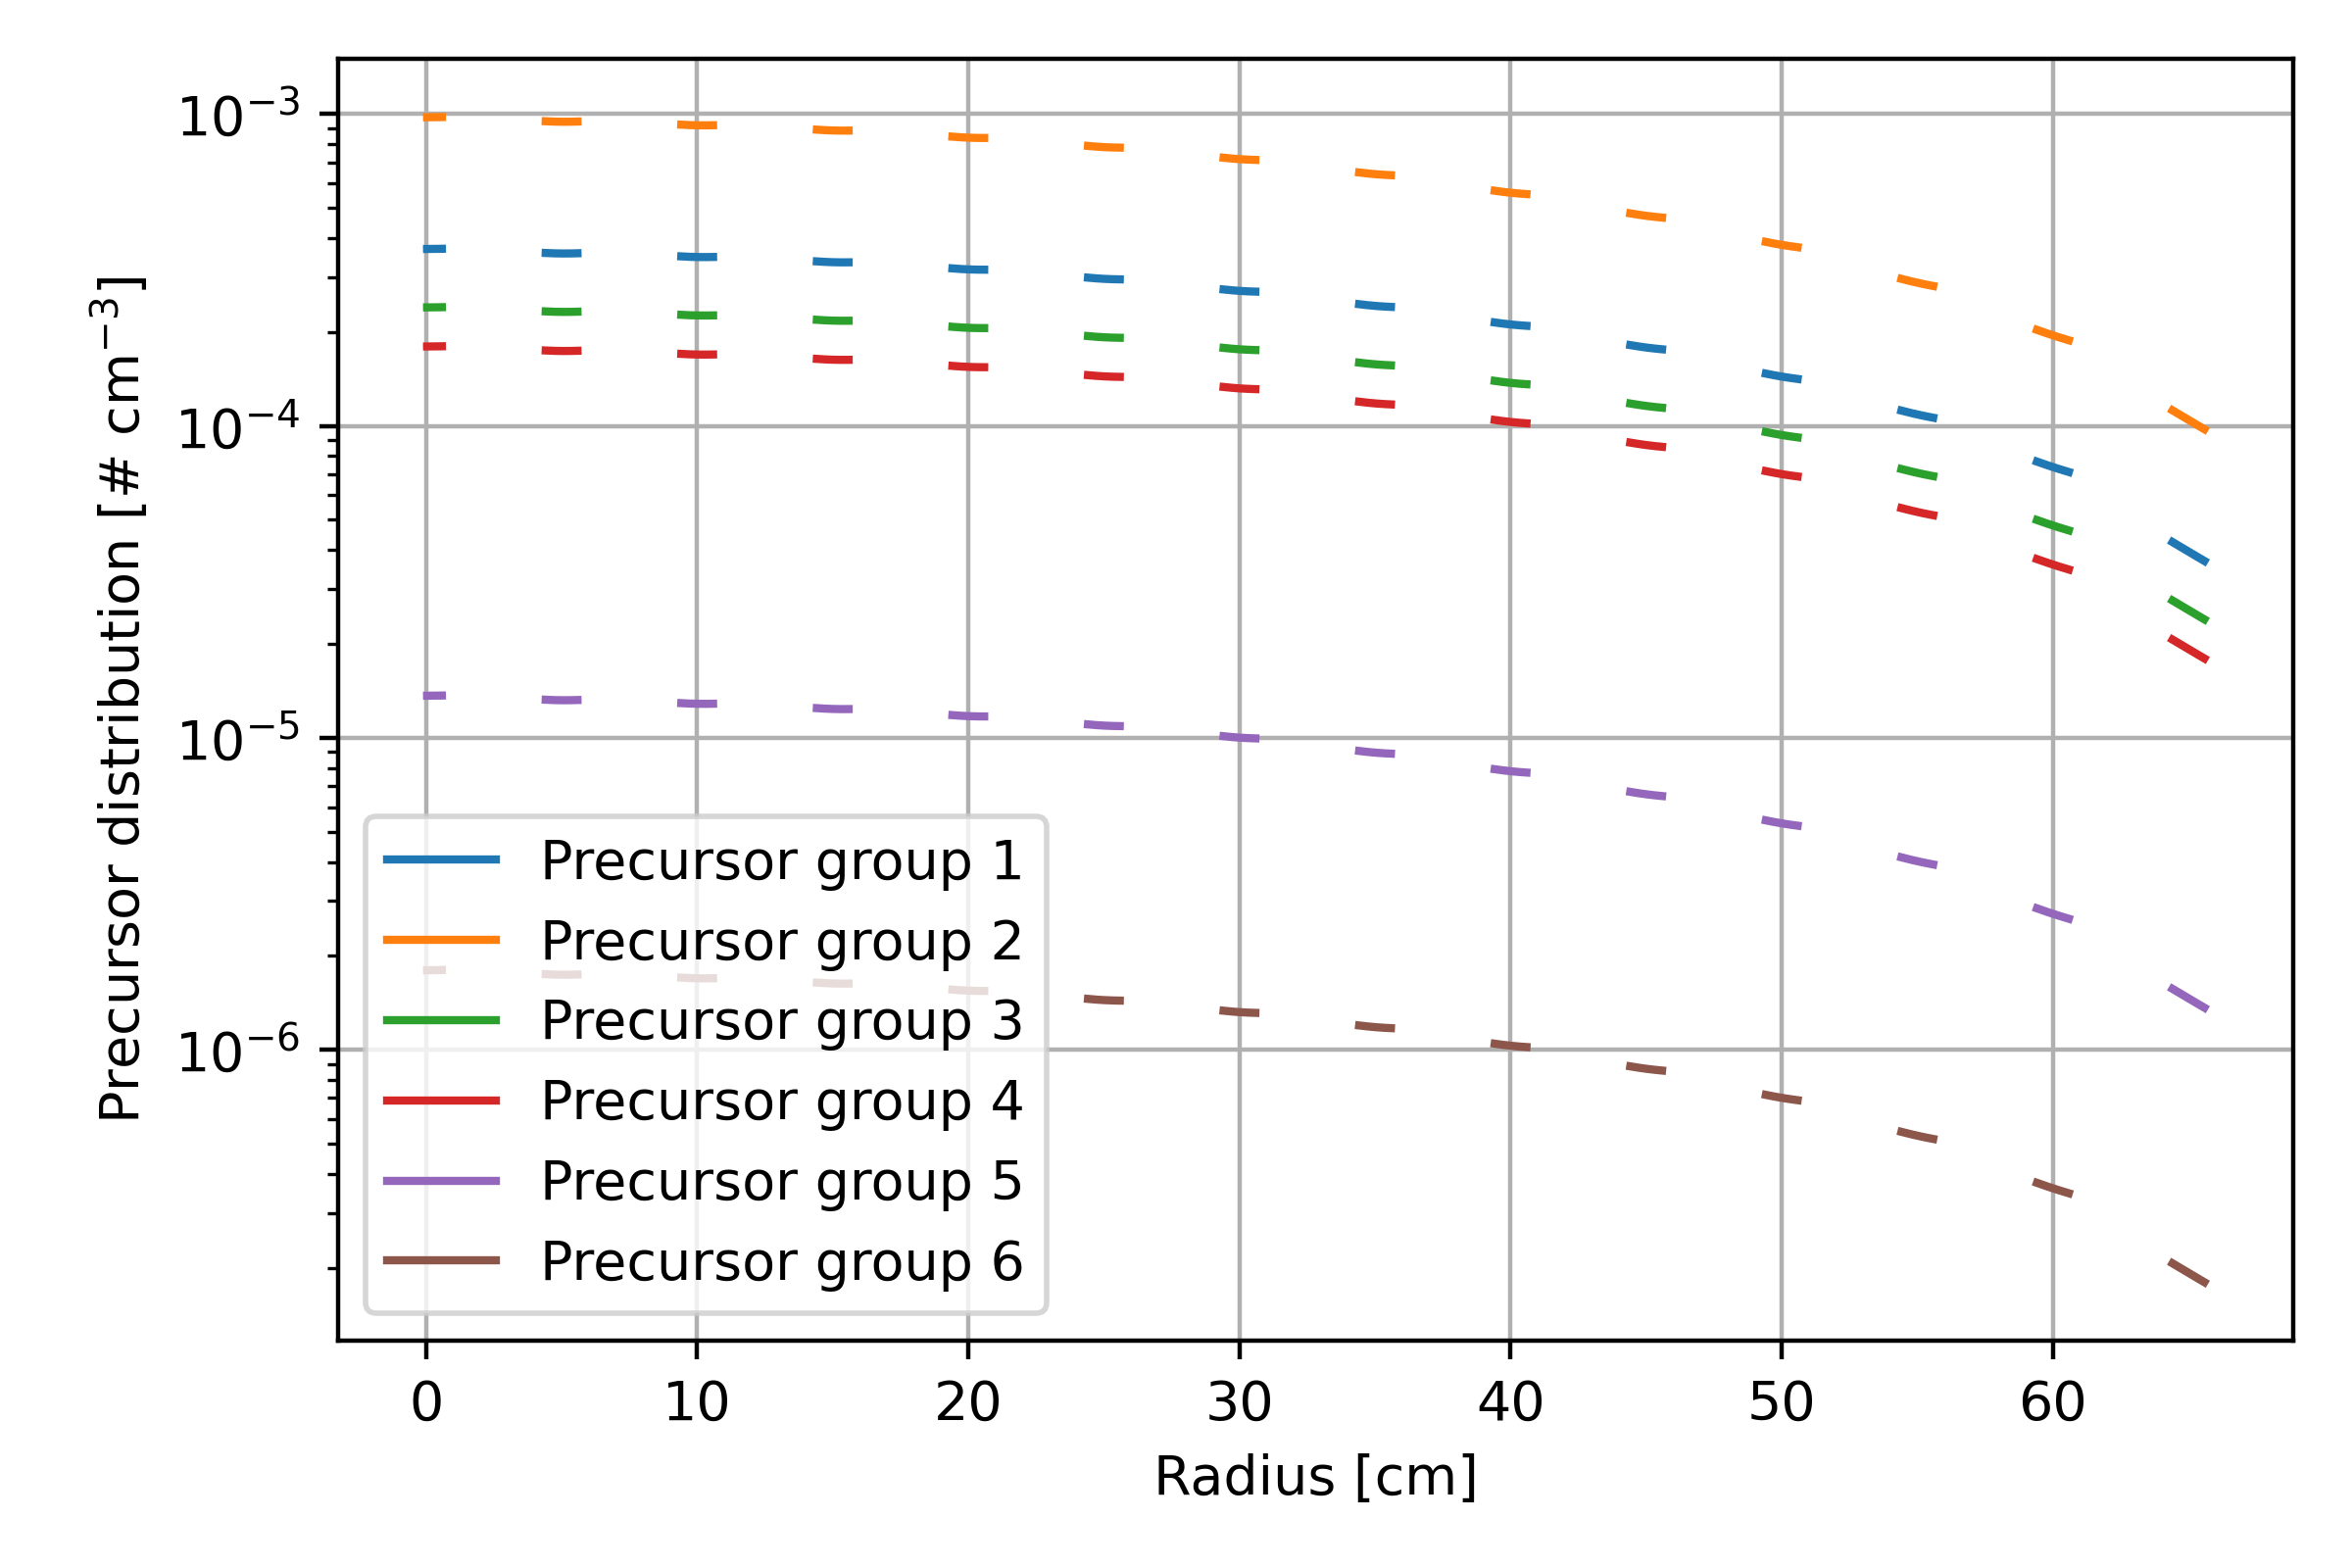
\includegraphics[width=\columnwidth]{midplane_pre}
      \caption{Normalized midplane \gls{DNP} distributions.}
      \label{fig:midplane-pre-dist}
    \end{subfigure}
    \caption{\gls{DNP} distribution from Moltres and ratios comparing QuasiMolto and
    Moltres models under static \gls{MSRE} conditions. Maximum relative difference $\approx 0.1 \%$.}
    \label{fig:centerline-pre}
  \end{figure}
  \begin{itemize}
    \item Perfect overlap in centerline and midplane DNP distributions between Moltres and QuasiMolto.
  \end{itemize}
\end{frame}

\begin{frame}[noframenumbering]
  \frametitle{Backward-Facing Step Flow Validation Test Results}
  \begin{columns}
    \column{11.5cm}
    \begin{figure}[htb]
      \centering
      \hfill
      \begin{subfigure}[t]{0.24\columnwidth}
        \centering
        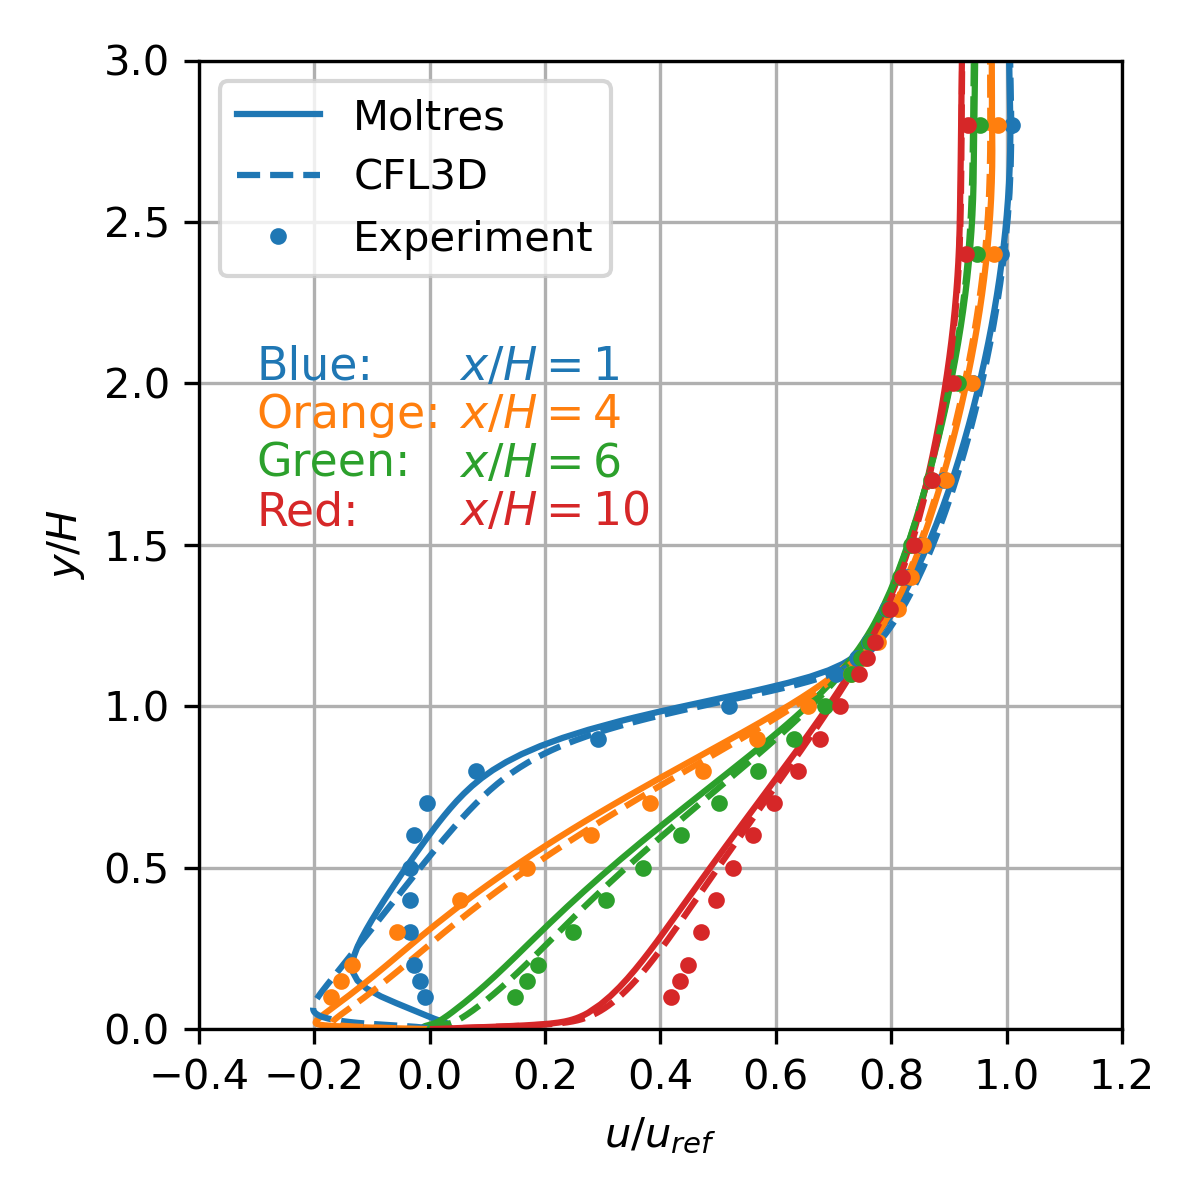
\includegraphics[width=\columnwidth]{bfs_downstream_vel}
        \caption{Normalized velocity distributions downstream of step.}
        \label{fig:bfs-downstream}
      \end{subfigure} %\hfill \\
  %    \centering
      \hfill
      \begin{subfigure}[t]{0.24\columnwidth}
        \centering
        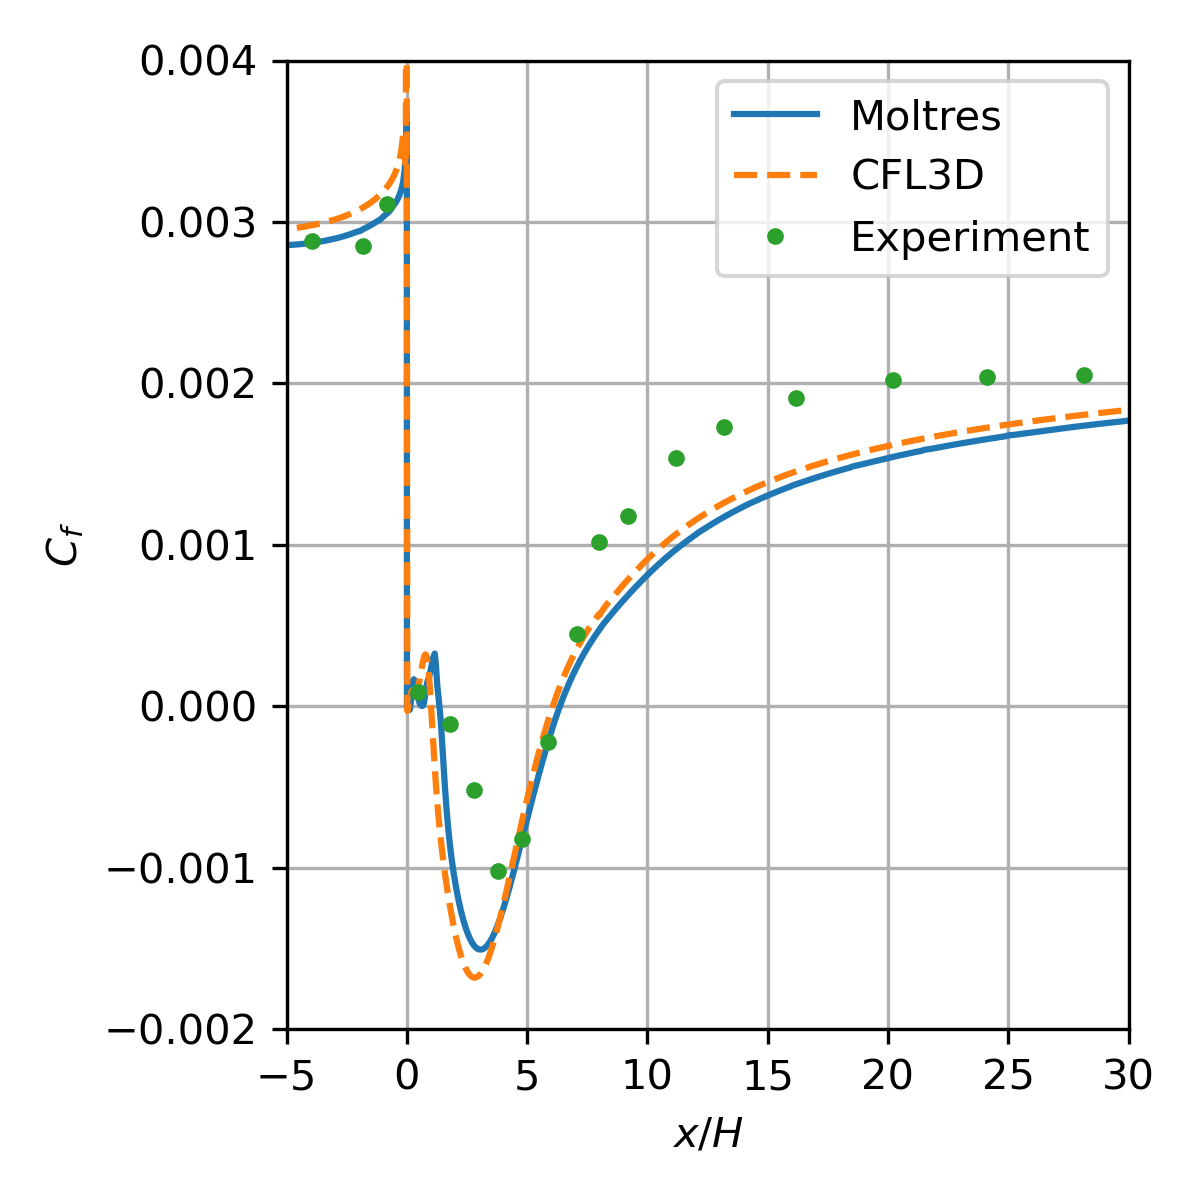
\includegraphics[width=\columnwidth]{bfs_cf}
        \caption{Skin friction coefficient along the bottom wall.}
        \label{fig:bfs-cf}
      \end{subfigure}
      \hfill
      \begin{subfigure}[t]{0.24\columnwidth}
        \centering
        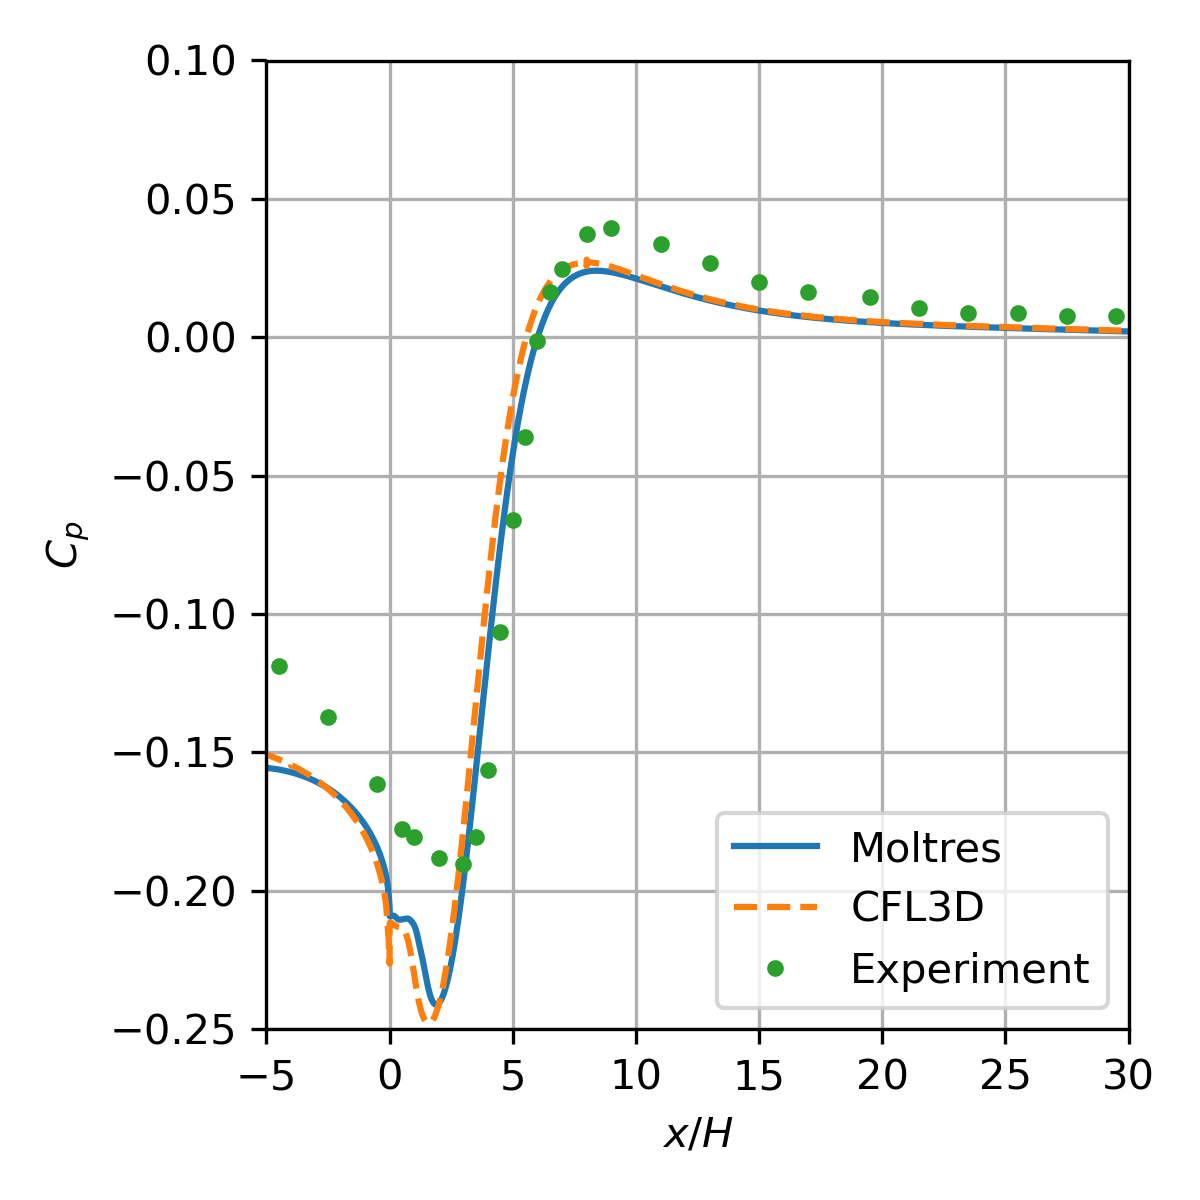
\includegraphics[width=\columnwidth]{bfs_cp}
        \caption{Skin pressure coefficient along the bottom wall.}
        \label{fig:bfs-cp}
      \end{subfigure}% \hfill \\
  %    \centering
      \begin{subfigure}[t]{0.24\columnwidth}
        \centering
        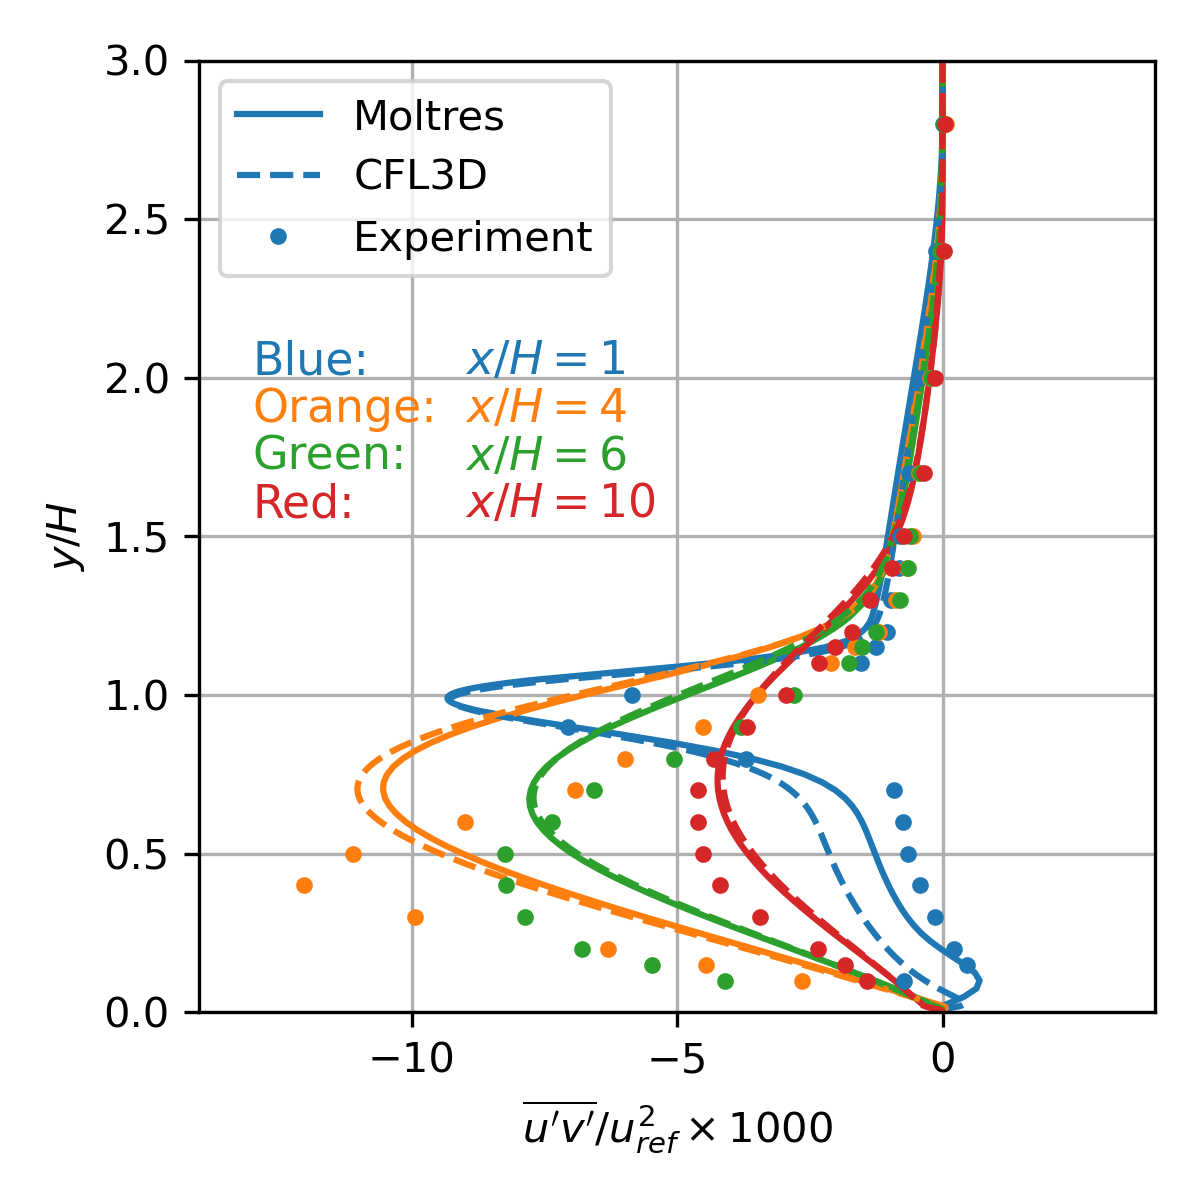
\includegraphics[width=\columnwidth]{bfs_stress}
        \caption{Normalized turbulent shear stress downstream
        of step.}
        \label{fig:bfs-stress}
      \end{subfigure}
      \caption{Comparison of backward facing step flow results against reference
      experimental data and computational data from CFL3D. $x/H$ values are normalized horizontal
      distances relative to the step.}
      \label{fig:bfs-plots}
    \end{figure}
  \end{columns}
  \begin{itemize}
    \item Minor discrepancies between numerical and experimental data typical of RANS-based turbulence models.
    \item Moltres provides better predictments along $x/H=1$ than CFL3D.
  \end{itemize}
\end{frame}

\begin{frame}[noframenumbering]
  \frametitle{Hybrid $S_N$-Diffusion Method: Theory}
  \textbf{Weak Formulation of the Multigroup SAAF $S_N$ Equations}
  \begin{gather}
    \shortintertext{Streaming term:}
    \sum^G_{g=1}\sum^{N_d}_{d=1}w_d\left(\hat{\Omega}_d\cdot\nabla\Psi^*_{g,d},\tau_g\hat{\Omega}
    \cdot\nabla\Psi_{g,d}-(1-\tau_g\Sigma_{t,g})\Psi_{g,d}\right)_\mathcal{D} \\
    \shortintertext{Collision term: }
    \sum^G_{g=1}\sum^{N_d}_{d=1}w_d\left(\Psi^*_{g,d},\Sigma_{t,g}\Psi_{g,d}\right)_\mathcal{D} \\
    \shortintertext{Scattering term:}
    \sum^G_{g=1}\sum^{N_d}_{d=1}w_d\left(\Psi^*_{g,d}+\tau_g\hat{\Omega}_d\cdot\nabla\Psi^*_{g,d},
    \sum^G_{g'=1}\sum^L_{l=0}\Sigma^{g'\rightarrow g}_{s,l}\sum^l_{m=-l}
    \frac{2l+1}{w}Y_{l,m}(\hat{\Omega}_d)\phi_{g',l,m}\right)_\mathcal{D} \\
    \shortintertext{Fission source term: }
    \sum^G_{g=1}\sum^{N_d}_{d=1}w_d\left(\Psi^*_{g,d}+\tau_g\hat{\Omega}_d\cdot\nabla\Psi^*_{g,d},
    \frac{1}{w}\frac{\chi_{p,g}(1-\beta)}{k}\sum^G_{g'=1}\nu\Sigma_{f,g'}\phi_{g'}\right)_\mathcal{D}
  \end{gather}
\end{frame}

\begin{frame}[noframenumbering]
  \frametitle{Hybrid $S_N$-Diffusion Method: Theory}
  \textbf{Weak Formulation of the Multigroup SAAF $S_N$ Equations}
  \begin{gather}
    \shortintertext{Delayed neutron source term:}
    \sum^G_{g=1}\sum^{N_d}_{d=1}w_d\left(\Psi^*_{g,d}+\tau_g\hat{\Omega}_d\cdot\nabla\Psi^*_{g,d},
    \frac{1}{w}\sum ^I_{i=1}\chi_{d,g}\lambda_i C_i\right)_\mathcal{D}
    \shortintertext{Boundary source term:}
    \begin{cases}
      \sum^G_{g=1}\sum^{N_d}_{d=1}w_d\left(\Psi^*_{g,d},
      \hat{\Omega}_d\cdot\hat{n}_b\Psi_{g,d}\right)_{\partial\mathcal{D}},
      & \hat{\Omega}\cdot\hat{n}_b>0,\vec{r}\in\partial\mathcal{D} \\
      \sum^G_{g=1}\sum^{N_d}_{d=1}w_d\left(\Psi^*_{g,d},
      \hat{\Omega}_d\cdot\hat{n}_b\Psi^\text{inc}_{g,d}\right)_{\partial\mathcal{D}},
      & \hat{\Omega}\cdot\hat{n}_b<0,\vec{r}\in\partial\mathcal{D}
    \end{cases} \label{eq:boundary-source} \\
    \shortintertext{Reflecting boundary term:}
    \begin{cases}
      \sum^G_{g=1}\sum^{N_d}_{d=1}w_d\left(\Psi^*_{g,d},
      \hat{\Omega}_d\cdot\hat{n}_b\Psi_{g,d}\right)_{\partial\mathcal{D}},
      & \hat{\Omega}\cdot\hat{n}_b>0,\vec{r}\in\partial\mathcal{D}_s \\
      \sum^G_{g=1}\sum^{N_d}_{d=1}w_d\left(\Psi^*_{g,d},
      \hat{\Omega}_d\cdot\hat{n}_b\Psi_{g,d_r}\right)_{\partial\mathcal{D}},
      & \hat{\Omega}\cdot\hat{n}_b<0,\vec{r}\in\partial\mathcal{D}_s
    \end{cases} \label{eq:reflecting-bc}
  \end{gather}
\end{frame}

\begin{frame}[noframenumbering]
  \frametitle{Hybrid $S_N$-Diffusion Method: Theory}
  \textbf{Weak Formulation of the Multigroup SAAF $S_N$ Equations}
  \begin{gather}
    \shortintertext{Void stabilization parameter \cite{wang_diffusion_2014}:}
    \tau_g =
    \begin{cases}
      \frac{1}{c\Sigma_{t,g}} \mbox{ for } ch\Sigma_{t,g} \geq \varsigma \\
      \frac{h}{\varsigma} \mbox{ for } ch\Sigma_{t,g} < \varsigma
    \end{cases}, \\
    \shortintertext{where}
    \begin{align*}
      h &= \mbox{mesh element size,} & \\
      c &= \mbox{maximum stabilization factor,} & \\
      \varsigma &= \mbox{void constant.} &
    \end{align*}
  \end{gather}
  $c=1$ and $\varsigma=0.5$ by default.
  \vspace{.2cm}

  The SAAF-$S_N$ equations require this stabilization scheme
  in near-void regions where $\Sigma_{t,g}$ is very small.
\end{frame}

\begin{frame}[noframenumbering]
%  \frametitle{Hybrid $S_N$-Diffusion Method: 1-D Neutronics Eigenvalue Simulations}
  \begin{columns}
    \column{5.5cm}
    \begin{figure}[htb!]
      \centering
      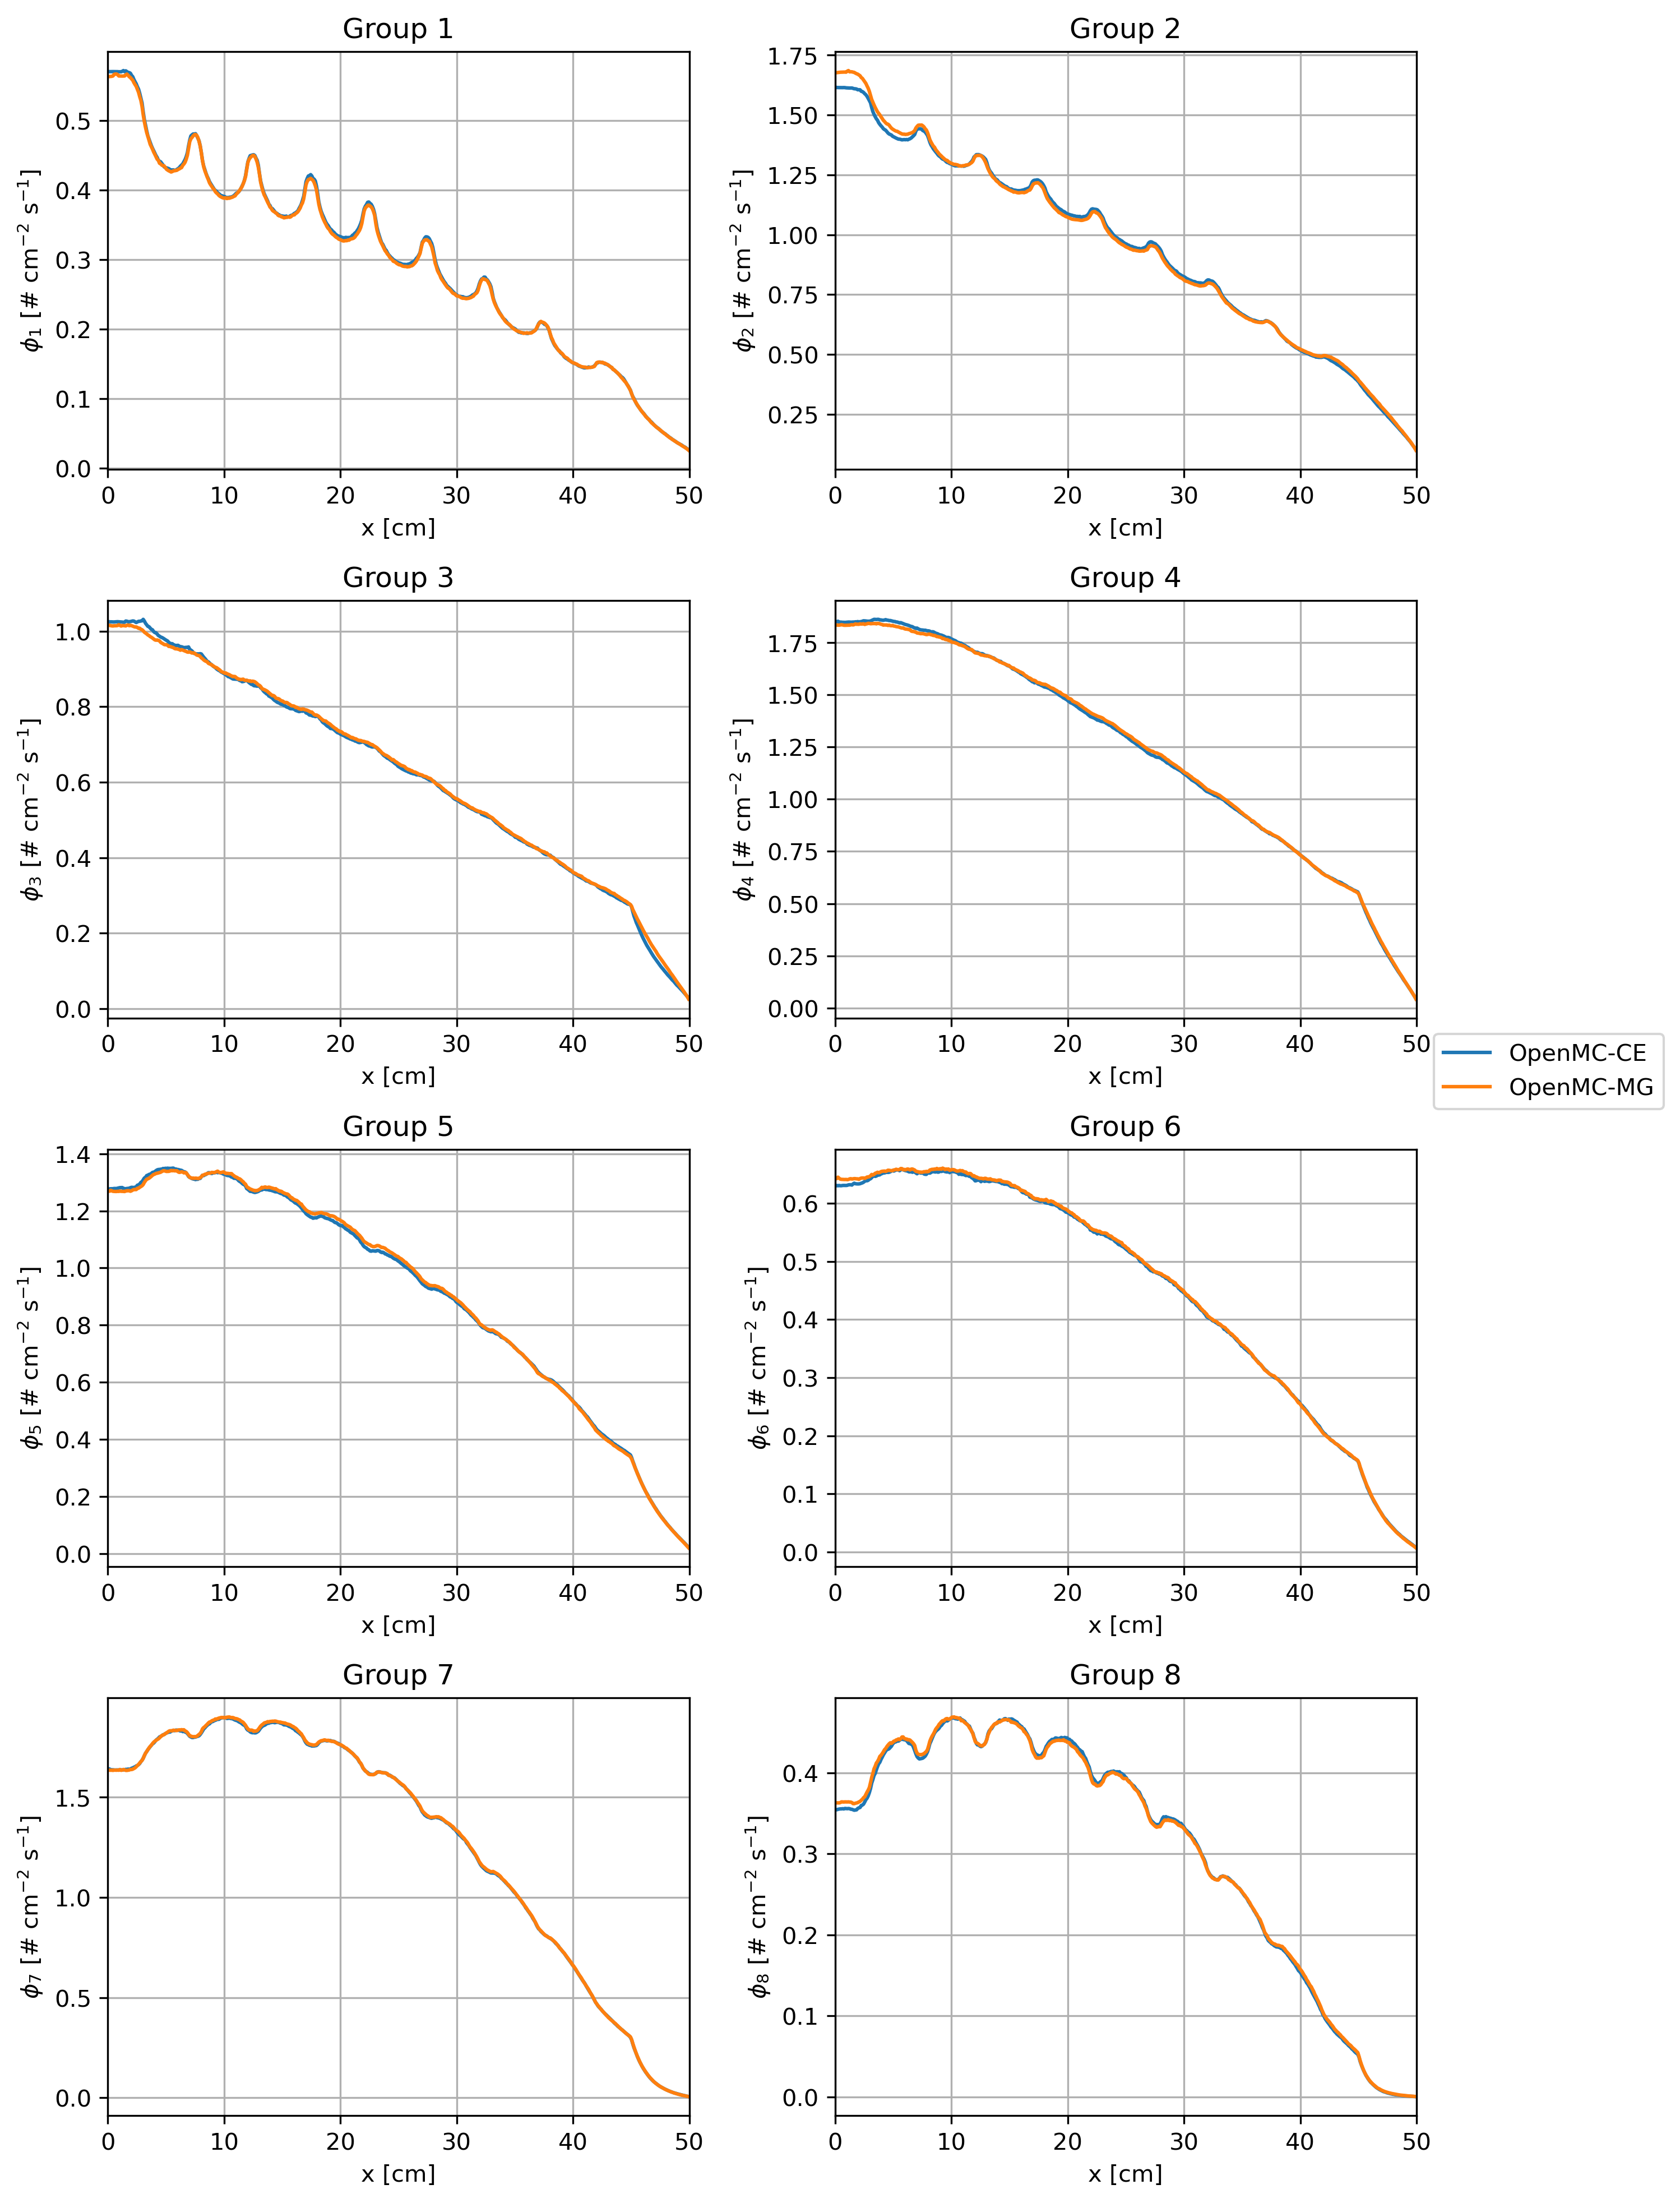
\includegraphics[width=\columnwidth]{case-3a-flux}
      \caption{Case 3a neutron group flux distributions from OpenMC-CE and OpenMC-MG.}
      \label{fig:3a-flux}
    \end{figure}
    \column{5.5cm}
    \begin{figure}[htb!]
      \centering
      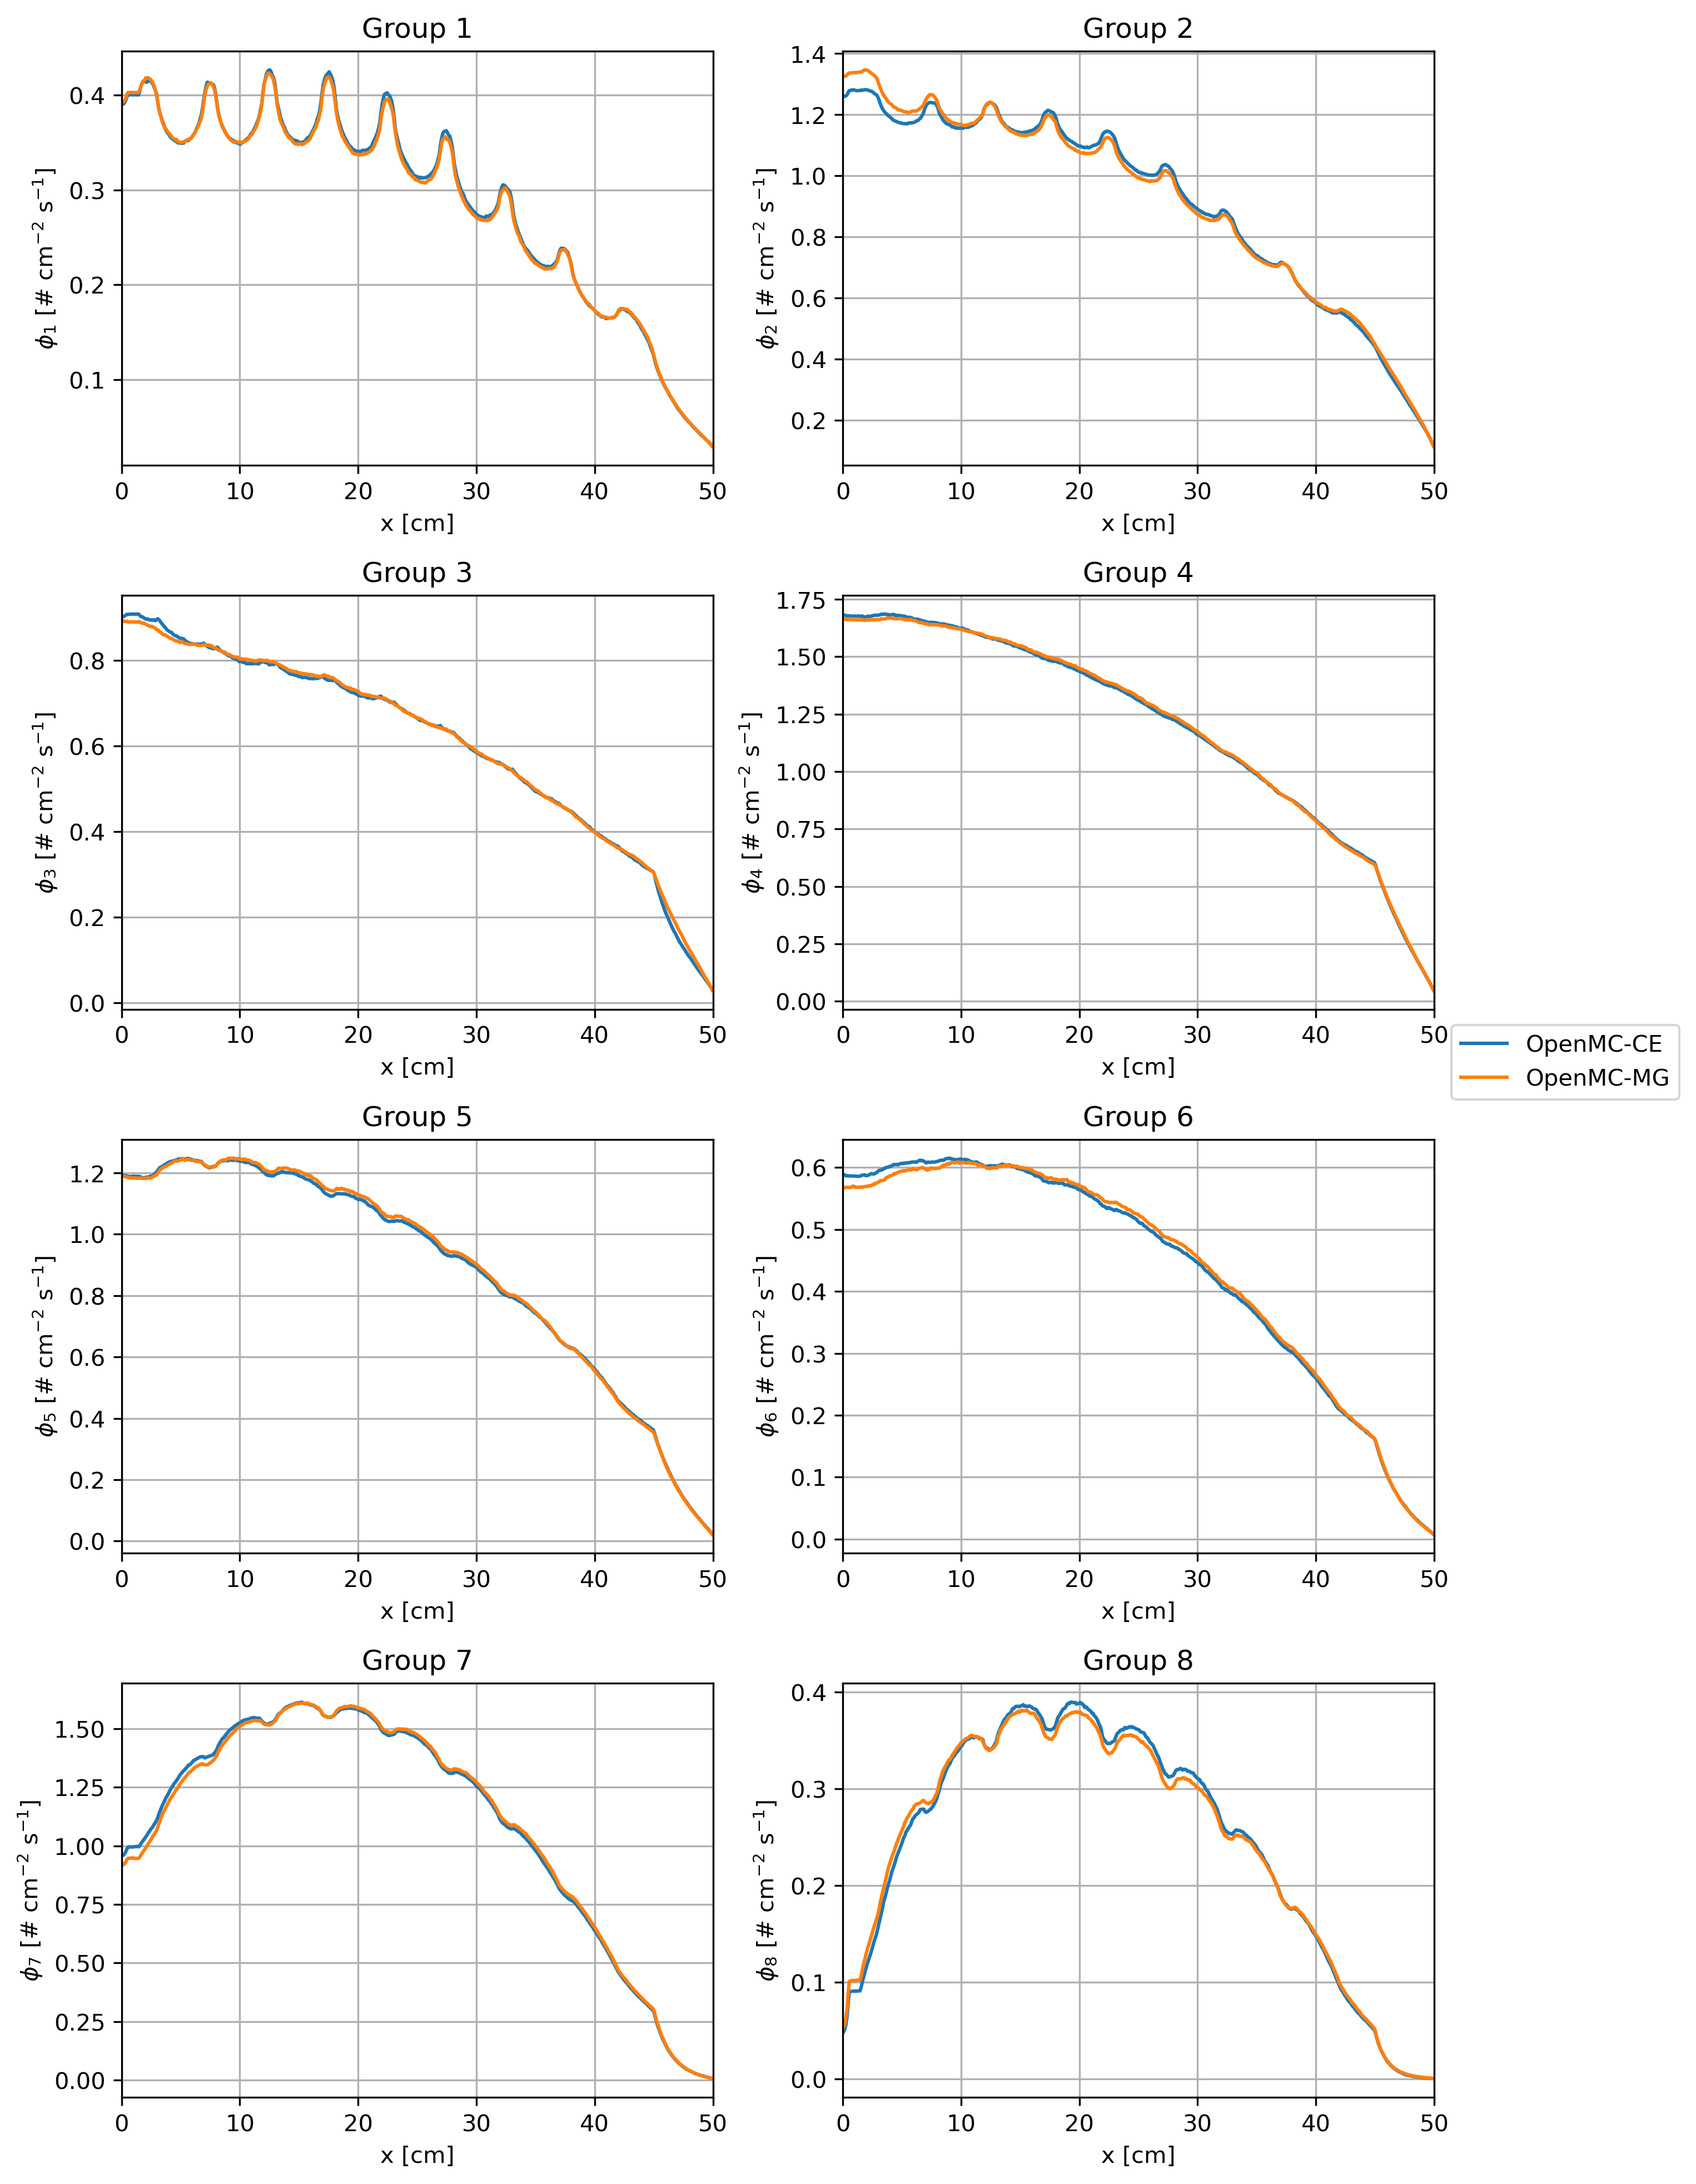
\includegraphics[width=\columnwidth]{case-3b-flux}
      \caption{Case 3b neutron group flux distributions from OpenMC-CE and OpenMC-MG.}
      \label{fig:3b-flux}
    \end{figure}
  \end{columns}
\end{frame}

\begin{frame}[noframenumbering]
%  \frametitle{Hybrid $S_N$-Diffusion Method: 1-D Neutronics Eigenvalue Simulations}
  \begin{columns}
    \column{5.5cm}
    \textbf{Case 3a Neutron Flux Distributions}
    \begin{itemize}
      \item The neutron diffusion and hybrid methods fare worse than the $S_8$ method at capturing
        the oscillatory flux pattern.
      \item The hybrid method performs better than the neutron diffusion method near $x=0$ cm where
        the correction region is situated.
    \end{itemize}
    \column{5.5cm}
    \begin{figure}[htb!]
      \centering
      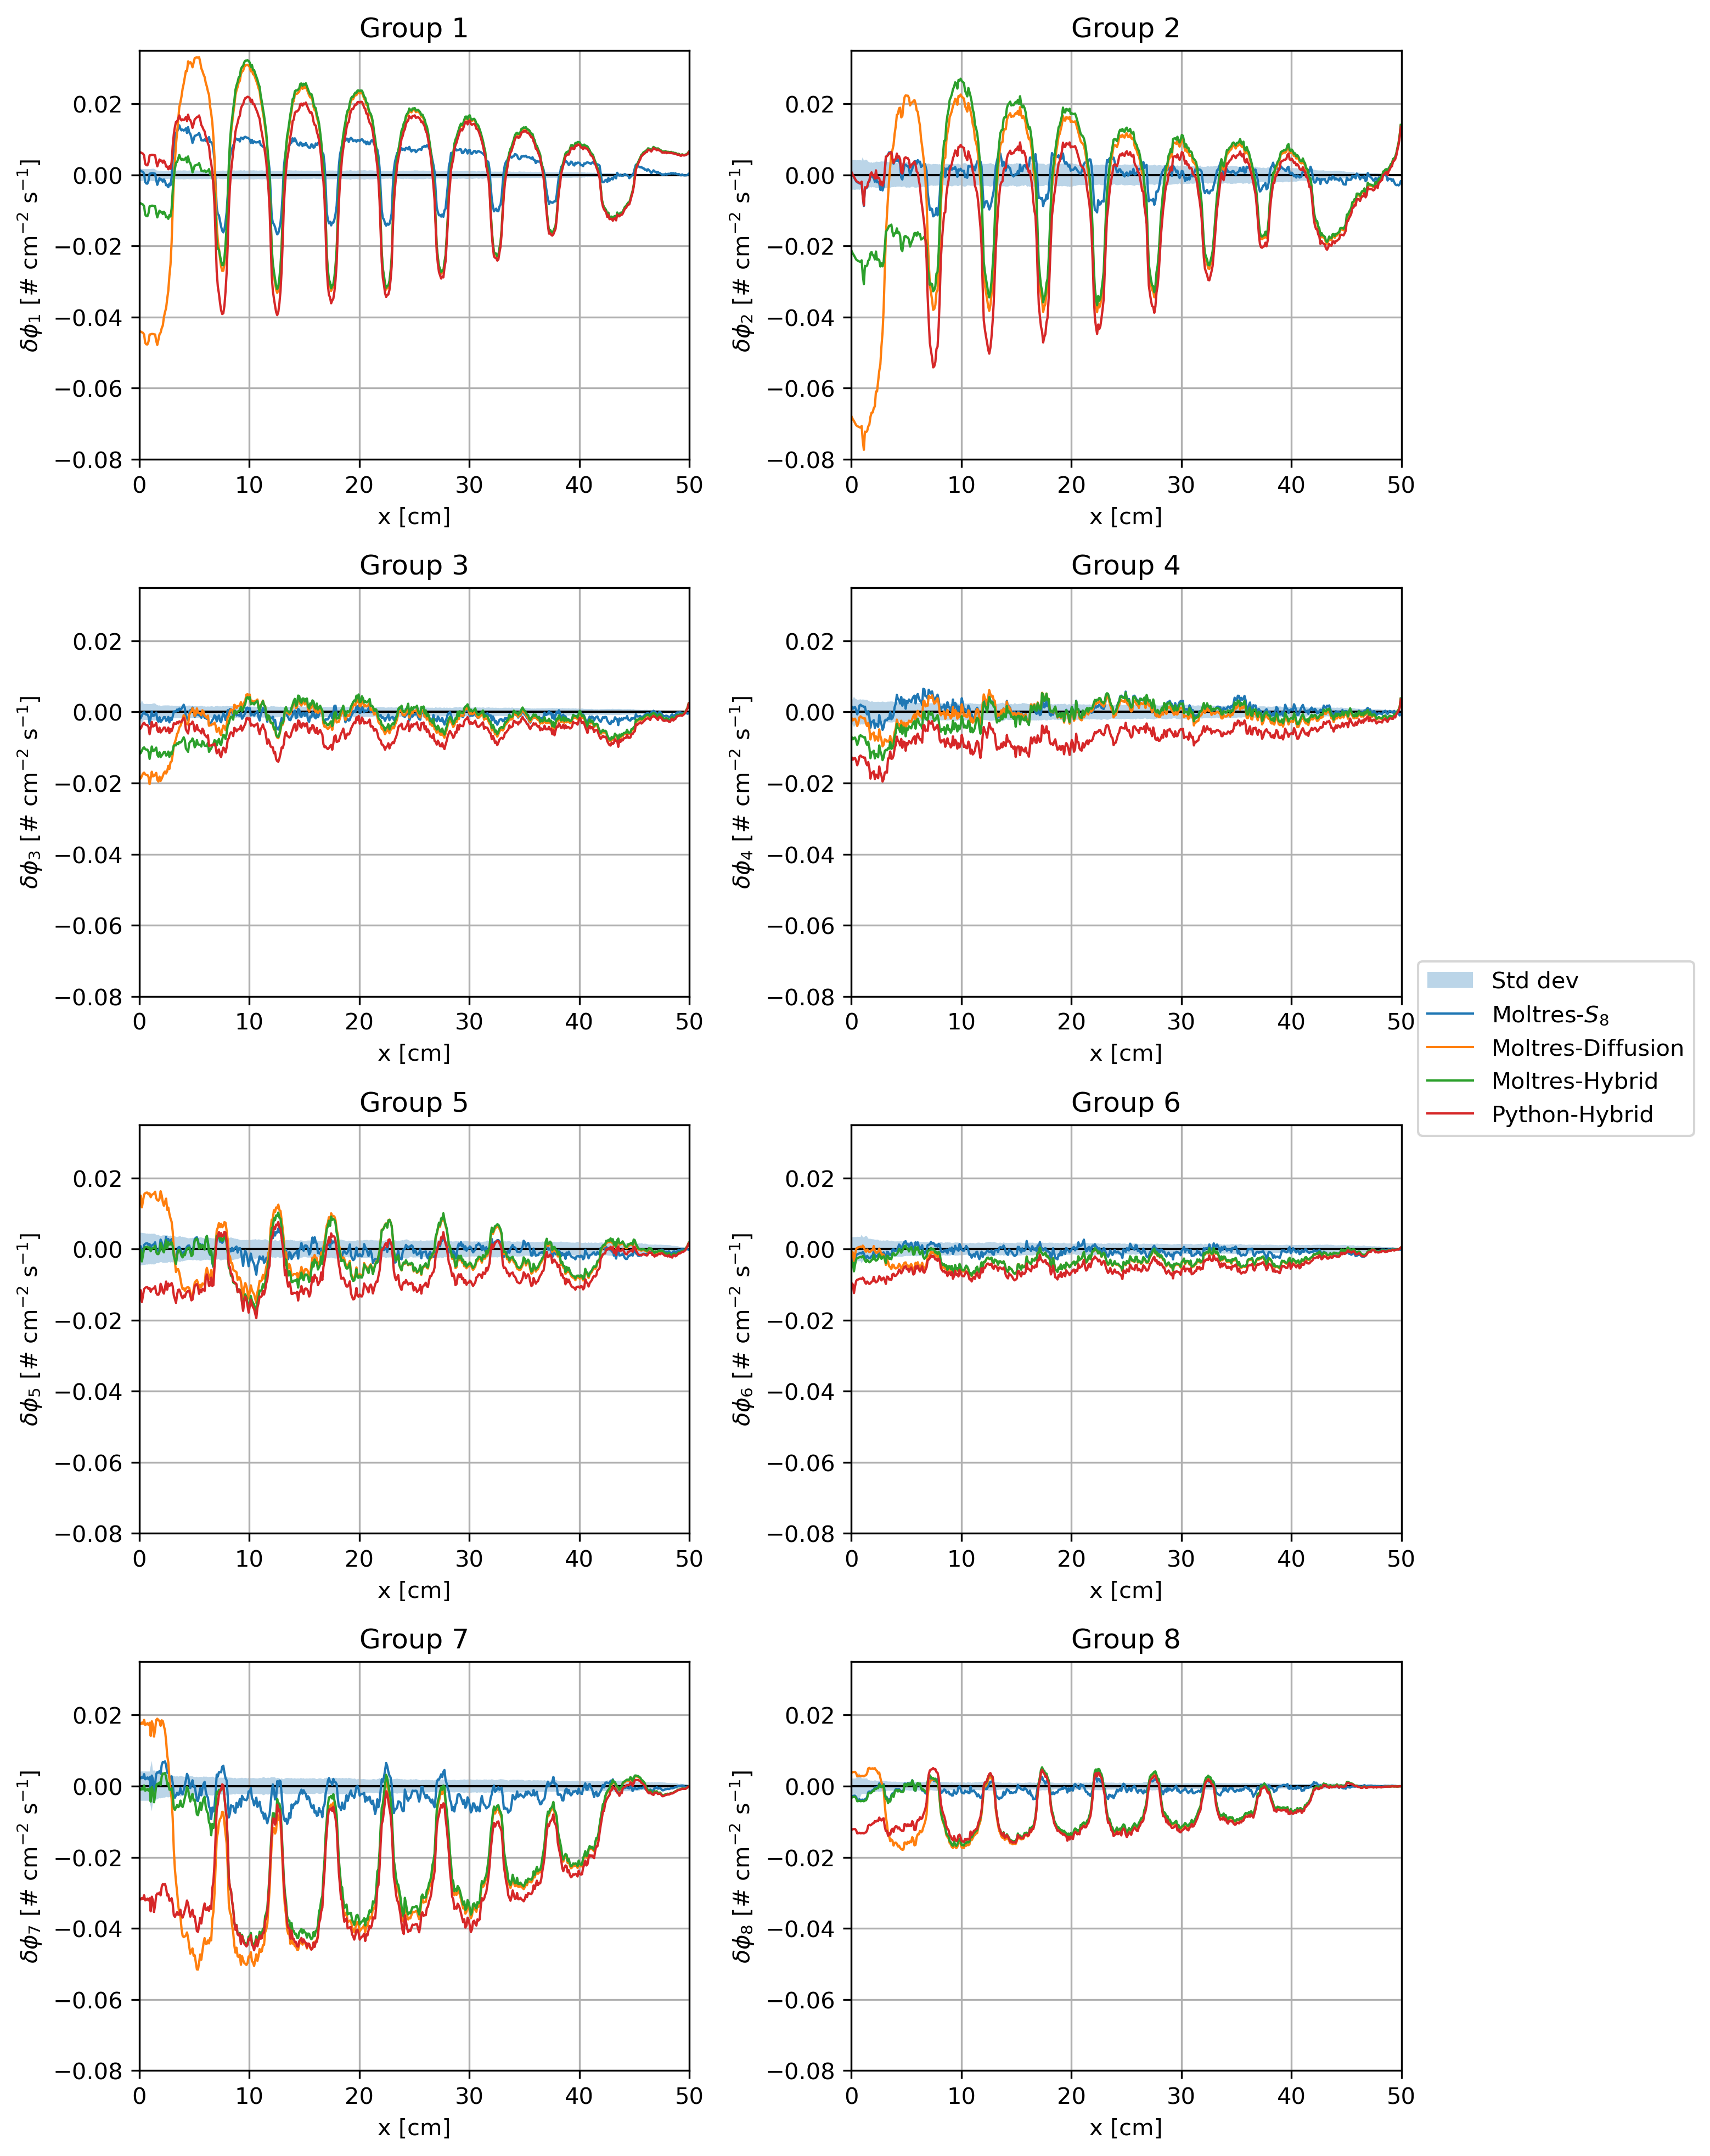
\includegraphics[width=.975\columnwidth]{case-3a-flux-diff}
      \caption{Absolute difference in neutron group flux distributions for Case 3a from Moltres-$S_8$,
      Moltres-diffusion, Moltres-hybrid, and Python-hybrid relative to OpenMC-MG.}
      \label{fig:3a-flux-diff}
    \end{figure}
  \end{columns}
\end{frame}

\begin{frame}[noframenumbering]
  \frametitle{Hybrid $S_N$-Diffusion Method: 1-D Neutronics Eigenvalue Simulations}
  \textbf{Impact of Correction Subregion Sizes on $k$}
  \begin{itemize}
    \item Minimizing the correction region size is essential for the hybrid method to be
      computationally efficient for time-dependent simulations.
    \item $k$ varies by up to 164 pcm for Case 3a and 109 pcm for Case 3b.
    \item The hybrid method $k$ value does not converge monotonically towards the $S_8$ method $k$ value,
      implying other sources of discrepancies.
  \end{itemize}
  \begin{figure}[h]
    \centering
    \begin{subfigure}[b]{0.49\columnwidth}
      \centering
      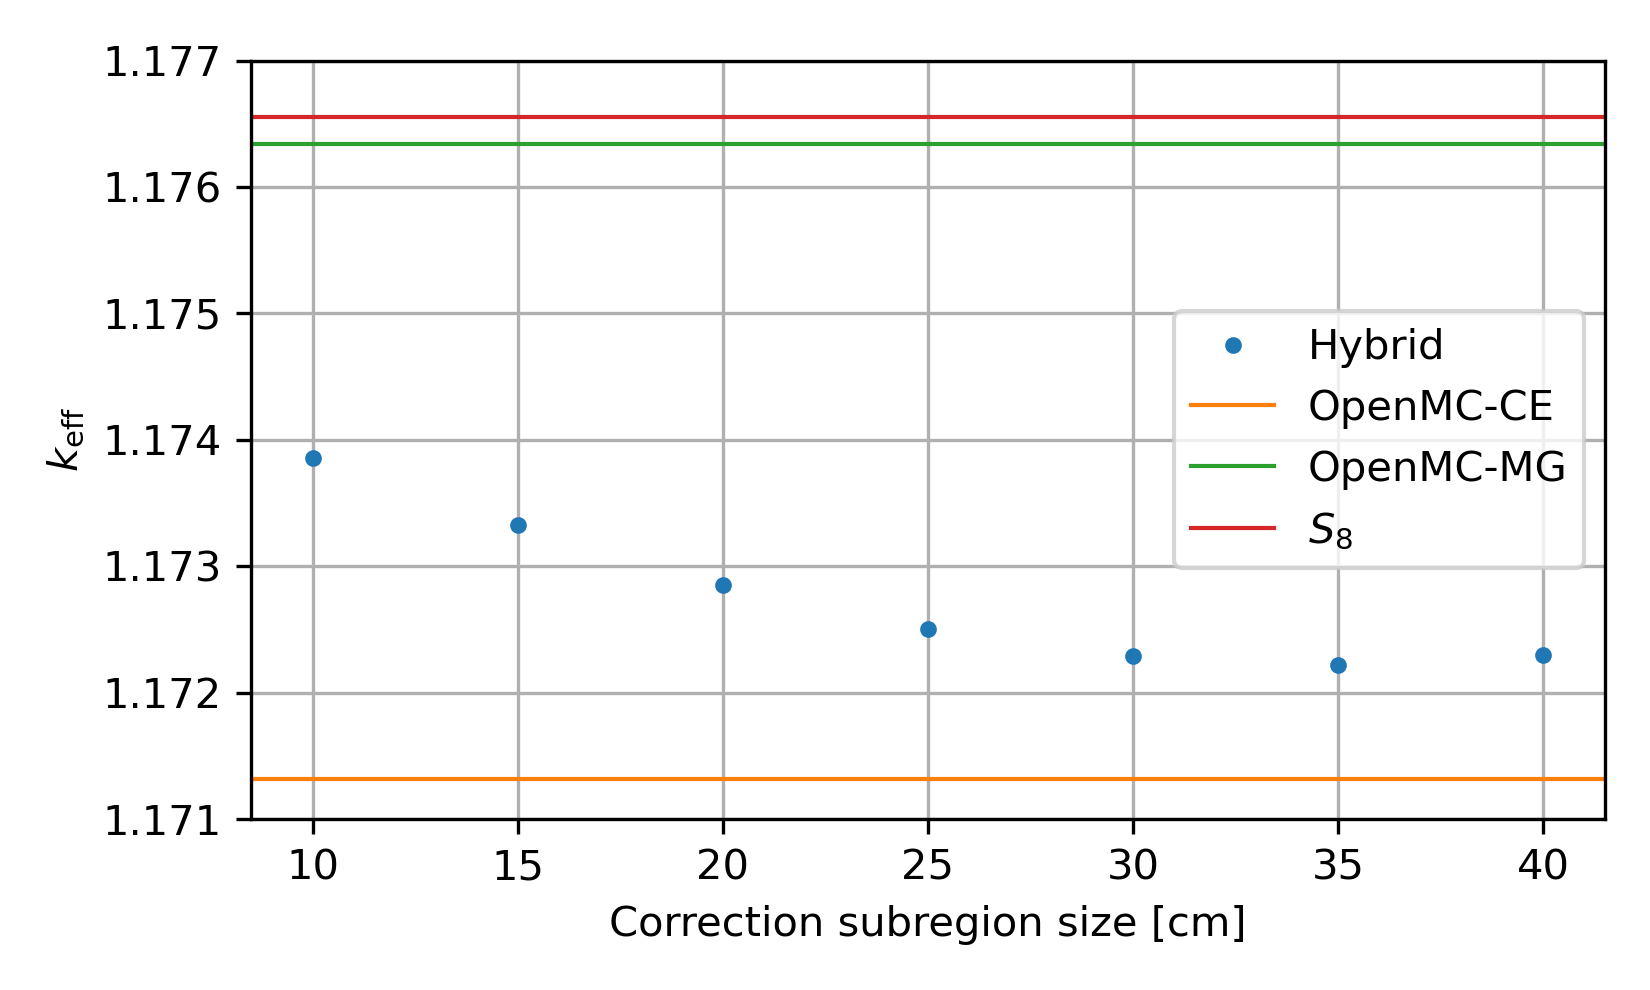
\includegraphics[width=\columnwidth]{correction-size-a-k}
      \caption{Case 3a}
      \label{fig:v1-size-a-k}
    \end{subfigure}
    \hfill
    \begin{subfigure}[b]{0.49\columnwidth}
      \centering
      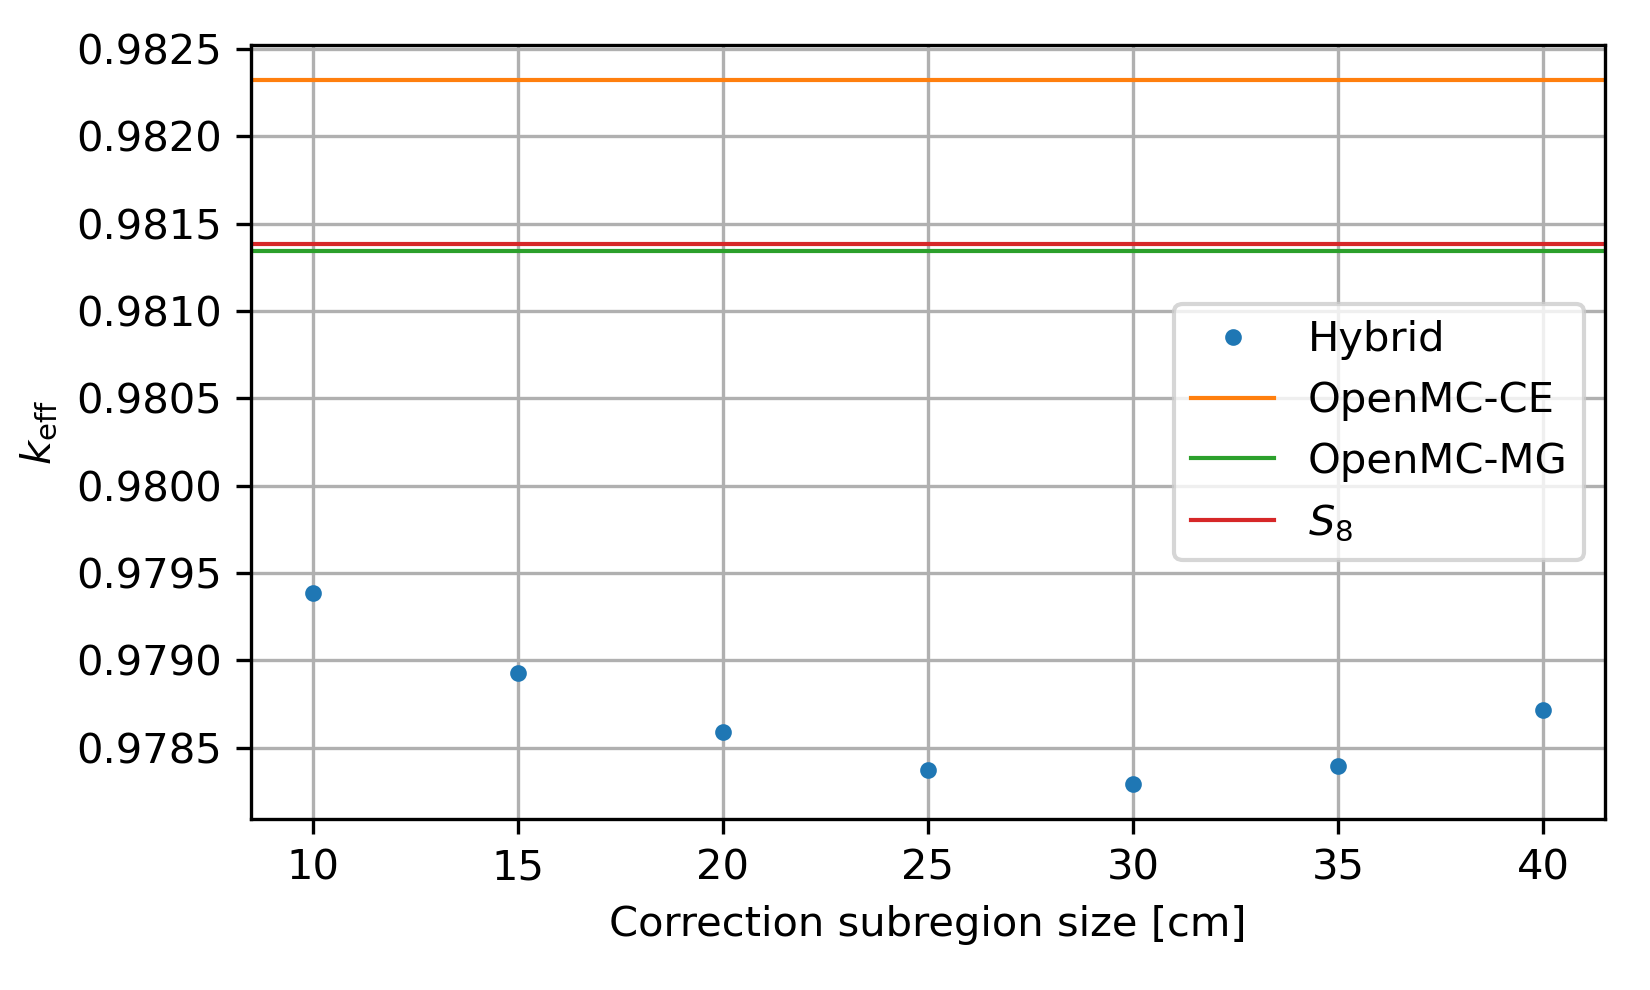
\includegraphics[width=\columnwidth]{correction-size-b-k}
      \caption{Case 3b}
      \label{fig:v1-size-b-k}
    \end{subfigure}
    \caption{$k_\text{eff}$ estimates from the hybrid method for Cases 3a and 3b with different
    correction subregion sizes. The horizontal lines indicate $k_\text{eff}$ estimates from the
    OpenMC-CE, OpenMC-MG, and $S_8$ methods.}
    \label{fig:v1-size-k}
  \end{figure}
\end{frame}

\begin{frame}[noframenumbering]
  \frametitle{Hybrid $S_N$-Diffusion Method: 1-D Neutronics Eigenvalue Simulations}
  \textbf{Relaxing the $S_N$ Convergence Tolerance}
  \begin{itemize}
    \item The hybrid $S_N$-diffusion method iteratively couples the neutron diffusion solver with
      the $S_N$ subsolver.
    \item Diffusion-based acceleration schemes for neutron transport methods typically do not
      require the neutron transport calculations to fully converge.
    \item Transport correction parameters tend to converge faster than scalar flux.
    \item Relaxing the $S_N$ subsolver convergence tolerance would provide computational savings to
      the hybrid method.
  \end{itemize}
\end{frame}

\begin{frame}[noframenumbering]
  \frametitle{Hybrid $S_N$-Diffusion Method: 3-D Neutronics Eigenvalue Simulations}
  \textbf{3-D Full-Core MSRE Model Details}
  \begin{itemize}
    \item Hybrid $S_6$-diffusion method
    \item $^{235}$U concentration at initial criticality
    \item Uniform temperature at 911 K
    \item Stabilization factor of $c=250$
    \item Void constant of $\varsigma=0.5$
    \item Uncorrected diffusion coefficient values capped at $D_g = 2.5$
  \end{itemize}
  \vspace{.2cm}

  These parameters are required for numerical stability in the air-filled control rod
  thimble region.
  \vspace{.2cm}

  All hybrid method results are compared with MSRE experimental data, the MSRE numerical benchmark
  report data (Serpent 2 model) \cite{fratoni_molten_2020}, and the OpenMC model in this work.
\end{frame}

\begin{frame}[noframenumbering]
  \frametitle{Hybrid $S_N$-Diffusion Method: 3-D Neutronics Eigenvalue Simulations}
  \textbf{MSRE at Initial Criticality}
  \begin{table}[htb]
    \centering
    \caption{$k_\text{eff}$ values from \gls{MSRE} experimental data, the \gls{MSRE} numerical
    benchmark \cite{fratoni_molten_2020}, and the OpenMC and Moltres models in this work.}
    \begin{tabular}{l S[table-format=1.5(2)]}
      \toprule
       & {$k_\text{eff}$} \\
       \midrule
      \gls{MSRE} experimental data & 1.00000(420) \\
      Serpent 2 (Numerical benchmark) & 1.02132(3) \\
      OpenMC (This work) & 1.01308(20) \\
      Hybrid (This work) & 1.01955 \\
      Diffusion (This work) & 1.01885 \\
      \bottomrule
    \end{tabular}
    \label{table:initial-crit}
  \end{table}

  \begin{itemize}
    \item The Serpent 2 benchmark model reports a $k_\text{eff}$ of 1.01093(3) after considering some
      of the geometrical modifications used in the OpenMC model.
    \item The hybrid and neutron diffusion models agree with the OpenMC model within 700 pcm.
  \end{itemize}
\end{frame}

\begin{frame}[noframenumbering]
  \frametitle{MSRE Rod Drop Experiment}
  \textbf{Rod Height}
  \begin{figure}[htb!]
    \centering
    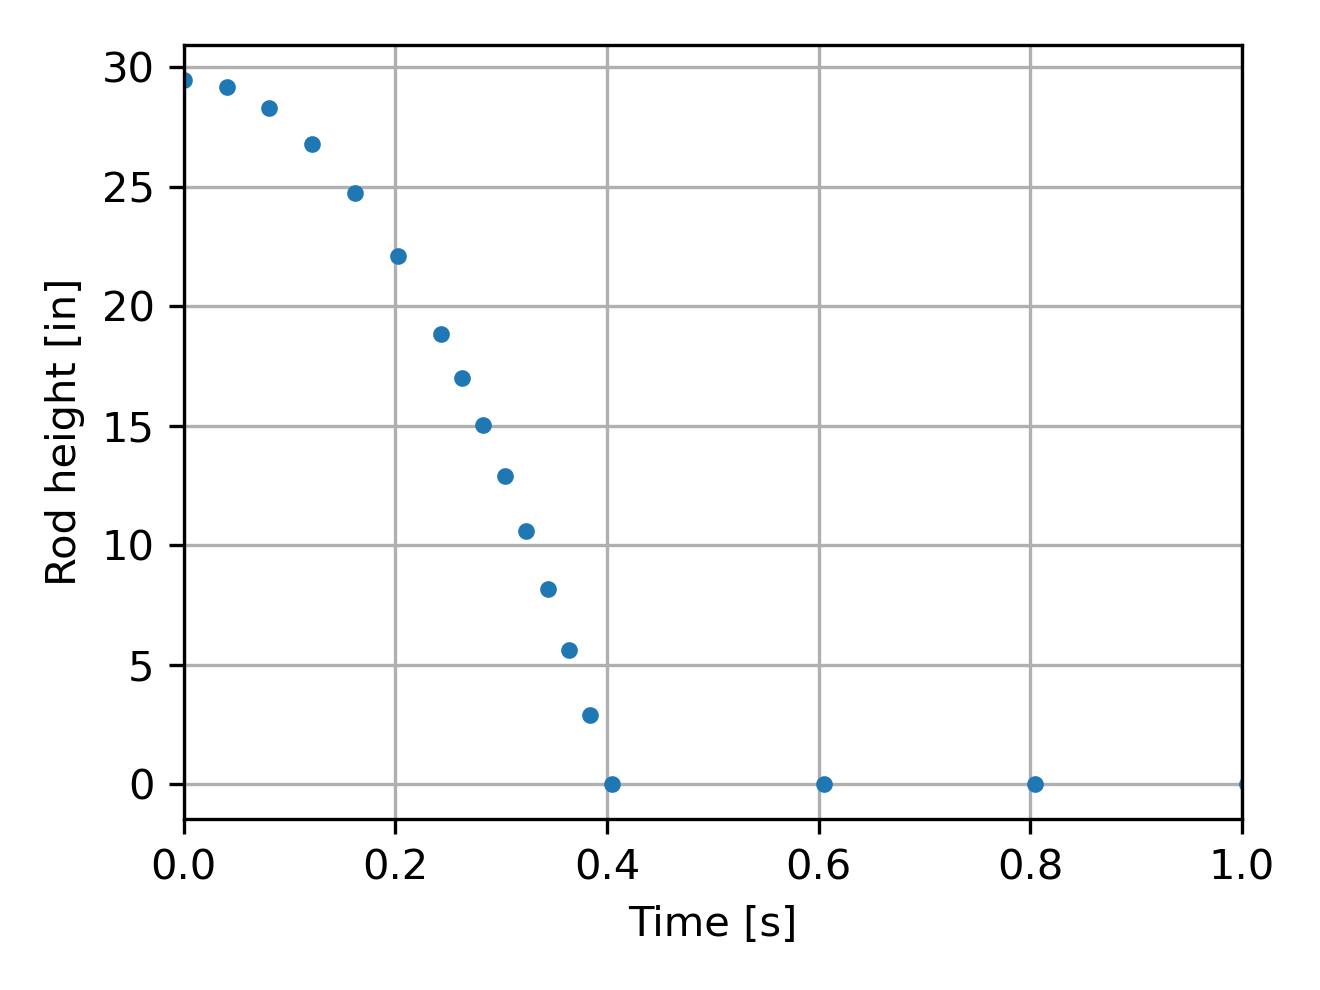
\includegraphics[width=0.7\columnwidth]{rod-height}
    \caption{Evolution of rod height evaluated at each timestep within the first second of the rod
    drop simulation. The rod reaches its fully inserted height at $t=0.4046$ s.}
    \label{fig:rod-height}
  \end{figure}
\end{frame}

%\begin{frame}[noframenumbering]
%  \frametitle{Molten Salt Reactor Designs}
%  \begin{columns}
%    \column{3cm}
%    \begin{figure}
%      \centering
%      \footnotesize
%      \includegraphics[width=\textwidth]{./images/msre-photo}
%      \caption{Graphite assembly for the Molten Salt Reactor Experiment
%      \cite{ornl_first-ever_2023}.}
%    \end{figure}
%    \column{7cm}
%    \begin{table}
%      \footnotesize
%      \centering
%      \caption{Thermal-spectrum MSR designs under active development.}
%      \begin{tabular}{l l}
%        \toprule
%        Reactor & Organization \\
%        \midrule
%        Integral Molten Salt Reactor & Terrestrial Energy \\
%        TMSR-LF & CAS (China) \\
%        Compact Molten Salt Reactor & Seaborg Technologies \\
%        Copenhagen Atomics Waste Burner & Copenhagen Atomics \\
%        \bottomrule
%      \end{tabular}
%    \end{table}
%    \begin{table}
%      \footnotesize
%      \centering
%      \caption{Fast-spectrum MSR designs under active development.}
%      \begin{tabular}{l l}
%        \toprule
%        Reactor & Organization \\
%        \midrule
%        Molten Chloride Fast Reactor & TerraPower \\
%        Molten Salt Fast Reactor & CNRS (France) \\
%        Stable Salt Reactor - Wasteburner & Moltex Energy \\
%        Molten Chloride Salt Fast Reactor & Elysium Industries \\
%        \bottomrule
%      \end{tabular}
%    \end{table}
%  \end{columns}
%\end{frame}
%
%\begin{frame}[noframenumbering]
%  \frametitle{V\&V Study 1: Verification of Moltres with the CNRS Benchmark}
%  \begin{table}
%      \caption{List of software packages and their corresponding model
%      specifications for the CNRS Benchmark simulations
%      \cite{tiberga_results_2020}.}
%      \centering
%      \footnotesize
%      \begin{tabular}{p{1.8cm} p{3.3cm} p{1.6cm} p{1cm} p{1.1cm}}
%          \toprule
%          Software & Institute & Numerical method & Mesh & Neutronics model \\
%          \midrule
%          OpenFOAM & Centre national de la recherche scientifique (CNRS) & Finite volume & 200$\times$200 \newline Non-uniform & $SP_1$ \& $SP_3$ \\
%          OpenFOAM & Politecnico di Milano (PoliMi) & Finite volume & 400$\times$400 \newline Uniform & Neutron diffusion \\
%          GeN-Foam & Paul Scherrer Institute (PSI) & Finite volume & 200$\times$200 \newline Non-uniform & Neutron diffusion \\
%          PHANTOM-$S_N$ DGFlows & Delft University of Technology (TUD) & Discontinuous finite \newline element & 50$\times$50 \newline Uniform & $S_2$ \& $S_6$ \\
%          Moltres (This work) & University of Illinois at Urbana-Champaign (UIUC) & Continuous \& discontinuous finite element & 200$\times$200 \newline Uniform & Neutron diffusion \\
%          \bottomrule
%      \end{tabular}
%      \label{table:software}
%  \end{table}
%\end{frame}
%
%\begin{frame}[noframenumbering]
%  \frametitle{Turbulence Models}
%  Numerous types of turbulence models exist at various levels of fidelity. From lowest to highest
%  computational complexity:
%  \begin{itemize}
%      \item RANS-based models
%      \begin{itemize}
%          \item Eddy viscosity models
%          \begin{itemize}
%              \item Algebraic models
%              \item One-equation
%              \item Two-equation models
%          \end{itemize}
%          \item \gls{RSM}
%      \end{itemize}
%      \item \gls{DES}
%      \item \gls{LES}
%      \item \gls{DNS}
%  \end{itemize}
%\end{frame}
%
%\begin{frame}[noframenumbering]
%  \frametitle{Turbulence Models}
%  \gls{RANS}-based models are based on the RANS equations obtained by applying time-averaging on
%  the fluid flow equations:
%  \begin{gather}
%      \frac{\partial U_i}{\partial t} + U_j \frac{\partial u_i}{\partial x_j} =
%      -\frac{1}{\rho} \frac{\partial P}{\partial x_i} + \nu \nabla^2 U_i -
%      \frac{\partial \langle u_i u_j \rangle}{x_j}
%      \shortintertext{where}
%      U = \mbox{ mean component,} \qquad u = \mbox{ fluctuating component.} \nonumber
%  \end{gather}
%  Eddy viscosity models operate on the eddy viscosity hypothesis:
%  \begin{align}
%      \langle u_iu_j \rangle =& \frac{2}{3}k \delta_{ij} - \nu_T \left(
%      \frac{\partial U_i}{\partial x_j} + \frac{\partial U_j}{\partial x_i}
%      \right)
%      \shortintertext{where}
%        \nu_T =& \mbox{ eddy viscosity.} \nonumber
%  \end{align}
%  The various eddy viscosity models mainly differ in their approach to the closure problem of
%  calculating the eddy viscosity.
%\end{frame}
%
%\begin{frame}[noframenumbering]
%  \frametitle{Control Rods in MSRs}
%  \begin{table}
%    \centering
%    \footnotesize
%    \caption{List of MSR designs which contain control rods.}
%    \begin{tabular}{l l}
%      \toprule
%      Reactor & Spectrum \\
%      \midrule
%      Molten Salt Reactor Experiment & Thermal \\
%      Integral Molten Salt Reactor & Thermal \\
%      TMSR-LF1 & Thermal \\
%      Liquid Fluoride Thorium Reactor & Thermal \\
%      Compact Molten Salt Reactor* & Thermal \\
%      Stable Salt Reactor - Wasteburner* & Fast \\
%      ThorCon Reactor* & Thermal \\
%      \bottomrule
%    \end{tabular}
%  \end{table}
%  Asterisks indicate MSR designs with ``control'' rods labeled as ``shutdown'' rods.
%\end{frame}
